\documentclass[11pt]{report}
\usepackage{outline}
\usepackage{pmgraph}
\usepackage[normalem]{ulem}
\usepackage{graphicx}
\usepackage[space]{grffile}
\usepackage{subcaption}
\usepackage{float}
\usepackage{hyperref}
\usepackage{enumitem}
\usepackage{pifont}
\hypersetup{
    colorlinks=true,
    linkcolor=blue,
    filecolor=magenta,      
    urlcolor=cyan,
}

\title{\textbf{CMPE 537 - Computer Vision} \\ Assignment - 1}
\author{Abdullah Atakan Güney}
\date{\today}
%--------------------Make usable space all of page
\setlength{\oddsidemargin}{0in}
\setlength{\evensidemargin}{0in}
\setlength{\topmargin}{0in}
\setlength{\headsep}{-.25in}
\setlength{\textwidth}{6.5in}
\setlength{\textheight}{8.5in}
%--------------------Indention
\setlength{\parindent}{1cm}

\begin{document}
%--------------------Title Page
\maketitle

\newpage

\tableofcontents

\newpage

\chapter{Task-1}
\section{Determining Color Channels}

In this part of the Assignment I have split the original image into RGB channels, and converted color-space to HSV and split into H, S, and V channels. After that, I have plotted both original RGB, and HSV images and I also plotted each channel separately with their intensity values mapped in to range from 0 to 255.

\begin{figure}
    \centering
    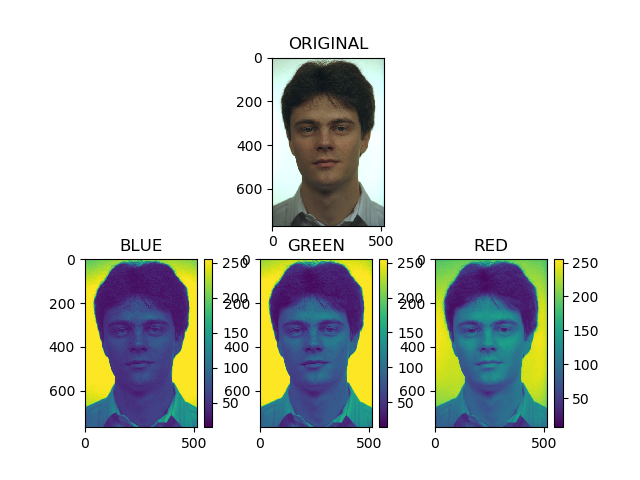
\includegraphics[height=0.4\textheight]{Task 1 Plots/RGB_plots.png}
    \caption{RGB plots for img\_001.jpg}
    \label{fig:rgb_all}
\end{figure}

\begin{figure}
    \centering
    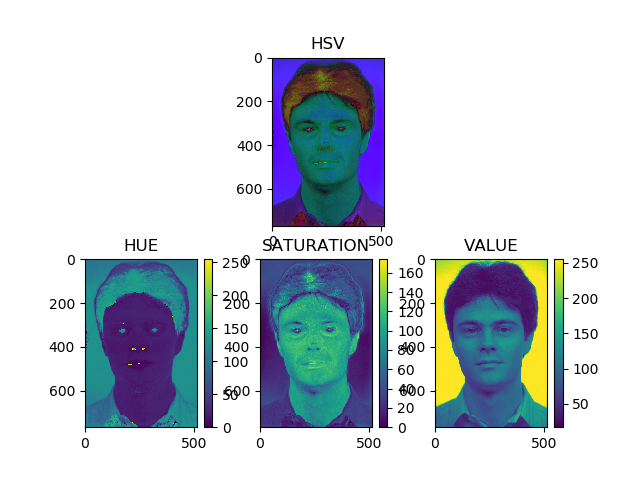
\includegraphics[height=0.4\textheight]{Task 1 Plots/HSV_plots.png}
    \caption{HSV plots for img\_001.jpg}
    \label{fig:hsv_all}
\end{figure}

\newpage

\section{Histograms of each channel}

For this part of the task, I have implemented a histogram function, which is based on numpy library. I have also checked my implementation of histogram function with 3 other ways to calculate histograms, one of them is numpy's histogram function.

\begin{figure}[H]
    \centering
    \begin{subfigure}{0.4\textwidth}
        \centering
        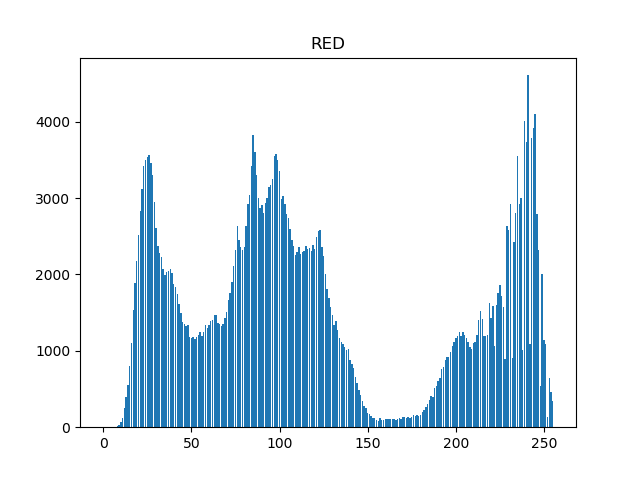
\includegraphics[width=0.9\textwidth]{Task 1 Plots/histogram_RED.png}
        \caption{RED}
        \label{fig:red_hist}
    \end{subfigure}
    \begin{subfigure}{0.4\textwidth}
        \centering
        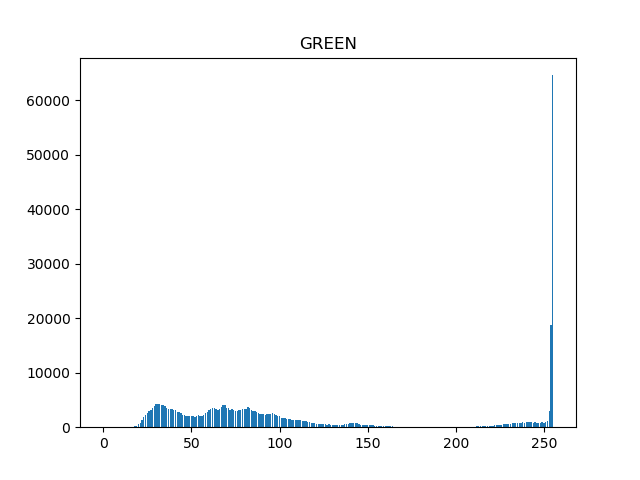
\includegraphics[width=0.9\textwidth]{Task 1 Plots/histogram_GREEN.png}
        \caption{GREEN}
        \label{fig:green_hist}
    \end{subfigure}
    \begin{subfigure}{0.4\textwidth}
        \centering
        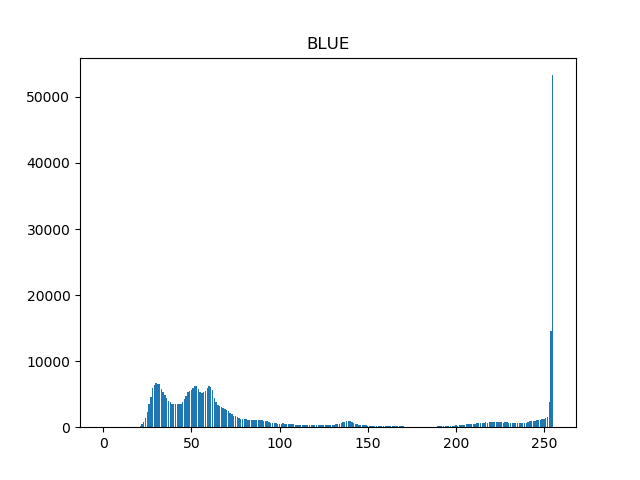
\includegraphics[width=0.9\textwidth]{Task 1 Plots/histogram_BLUE.png}
        \caption{BLUE}
        \label{fig:blue_hist}
    \end{subfigure}
    \caption{RGB Histograms}
    \label{fig:rgb_all_hist}
\end{figure}

\begin{figure}[H]
    \centering
    \begin{subfigure}{0.4\textwidth}
        \centering
        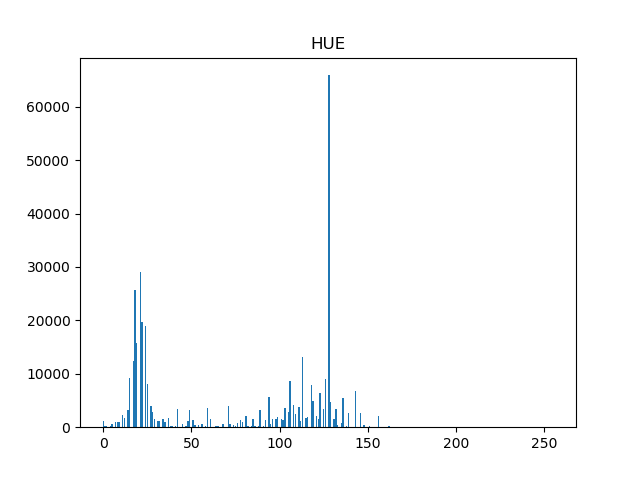
\includegraphics[width=0.9\textwidth]{Task 1 Plots/histogram_HUE.png}
        \caption{HUE}
        \label{fig:hue_hist}
    \end{subfigure}
    \begin{subfigure}{0.4\textwidth}
        \centering
        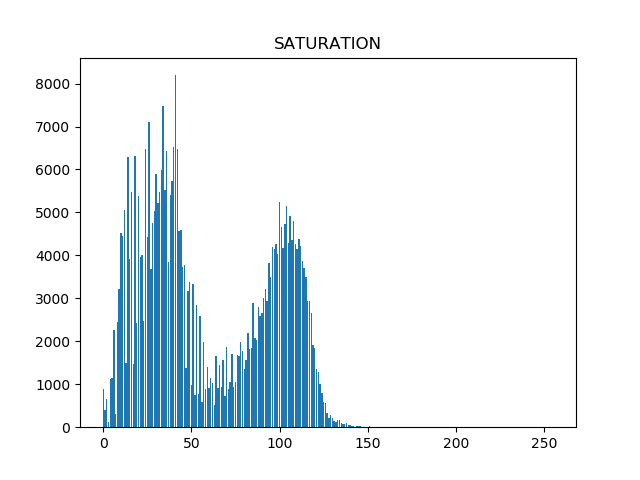
\includegraphics[width=0.9\textwidth]{Task 1 Plots/histogram_SATURATION.png}
        \caption{SATURATION}
        \label{fig:saturation_hist}
    \end{subfigure}
    \begin{subfigure}{0.4\textwidth}
        \centering
        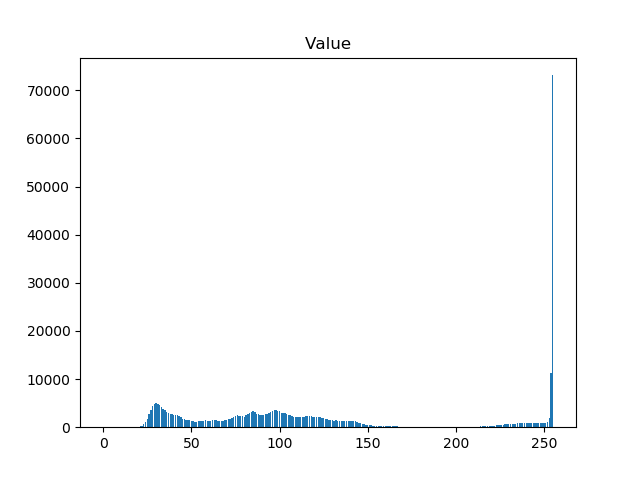
\includegraphics[width=0.9\textwidth]{Task 1 Plots/histogram_Value.png}
        \caption{VALUE}
        \label{fig:value_hist}
    \end{subfigure}
    \caption{HSV Histograms}
    \label{fig:hsv_all_hist}
\end{figure}

\newpage

\section{Conclusion of Task 1}
In this task, I have recognized that in different color spaces, different axes can be used for feature extraction for future applications. In RGB space, Green and Blue channels look like similar, on the other hand in HSV space Value is similar to Green and Blue, but Hue and Saturation are totally different, we can see the differences by looking at intensity images of these channels also.

\chapter{Task 2}
\section{Obtaining Binary Masks}

For this section, I have used ground truth images to obtain binary pixel masks. Let say, for a ground truth image with dimension $768 \times 512 \times 3$, I created an array with dimension $768 \times 512$ with full of zeros first, then I have set all the places to 255 that their corresponding place in the ground truth image is not $(0, 0, 0)$.

\begin{figure}[H]
    \centering
    \begin{subfigure}{0.3\textwidth}
        \centering
        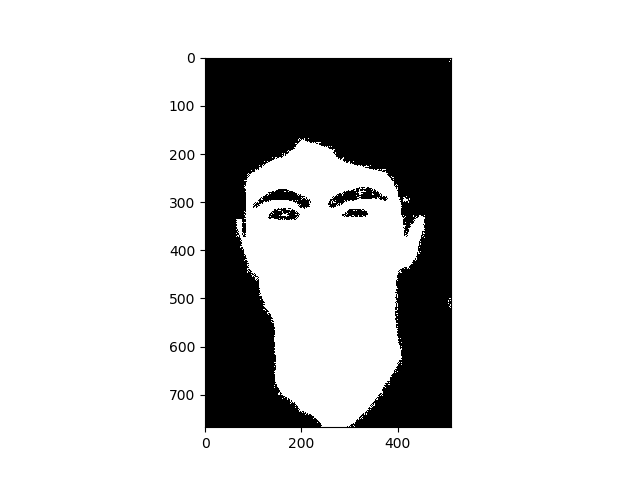
\includegraphics[width=\textwidth]{Task 2 Plots/bin_mask_001.png}
        \caption{image 001}
        \label{fig:binmask1}
    \end{subfigure}
    \begin{subfigure}{0.3\textwidth}
        \centering
        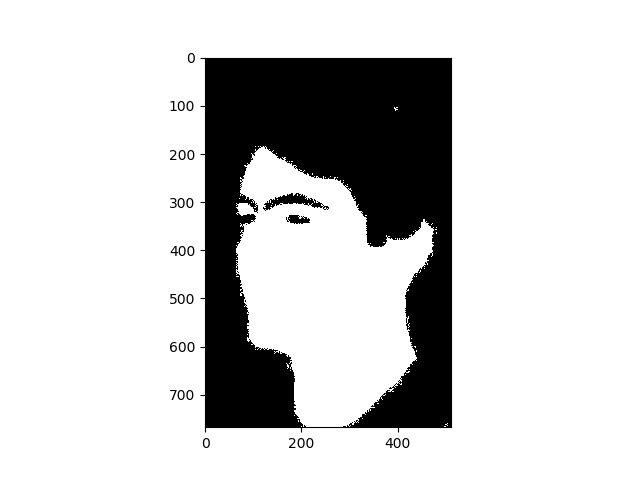
\includegraphics[width=\textwidth]{Task 2 Plots/bin_mask_002.png}
        \caption{image 002}
        \label{fig:binmask2}
    \end{subfigure}
    \begin{subfigure}{0.3\textwidth}
        \centering
        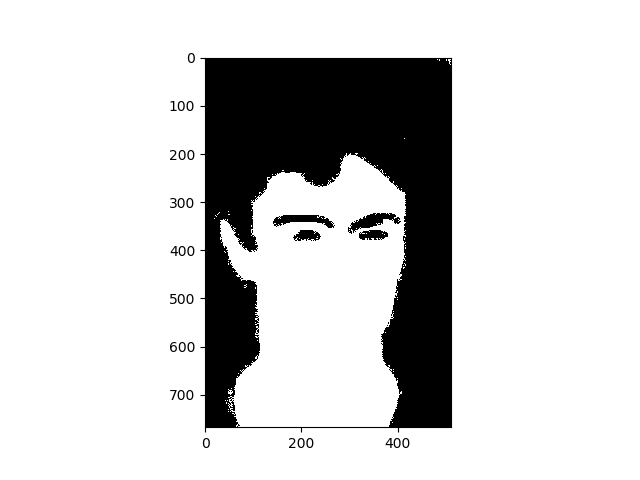
\includegraphics[width=\textwidth]{Task 2 Plots/bin_mask_003.png}
        \caption{image 003}
        \label{fig:binmask3}
    \end{subfigure}
    \begin{subfigure}{0.3\textwidth}
        \centering
        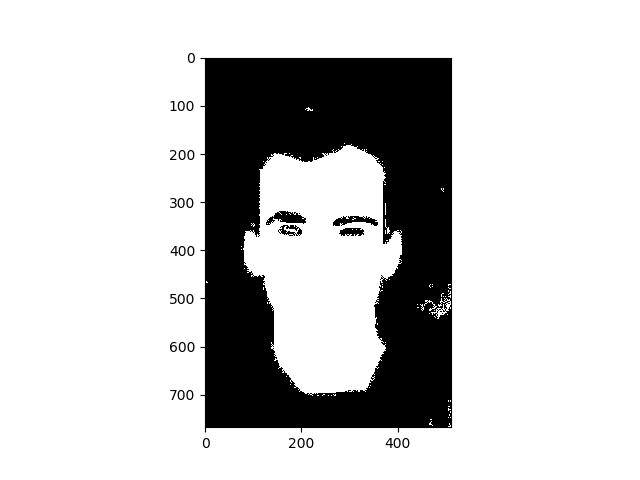
\includegraphics[width=\textwidth]{Task 2 Plots/bin_mask_004.png}
        \caption{image 004}
        \label{fig:binmask4}
    \end{subfigure}
    \begin{subfigure}{0.3\textwidth}
        \centering
        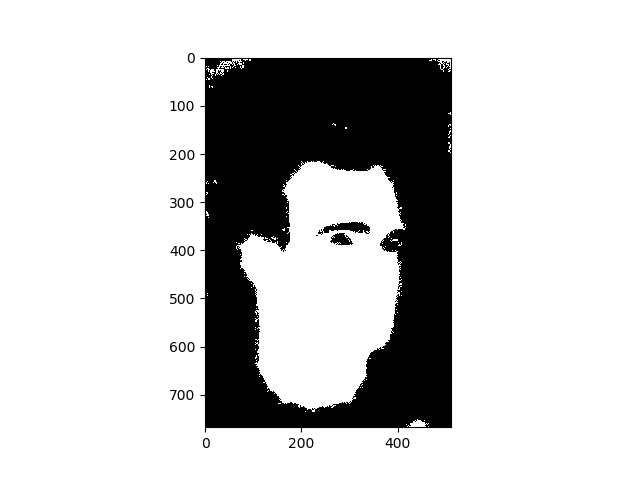
\includegraphics[width=\textwidth]{Task 2 Plots/bin_mask_005.png}
        \caption{image 005}
        \label{fig:binmask5}
    \end{subfigure}
    \begin{subfigure}{0.3\textwidth}
        \centering
        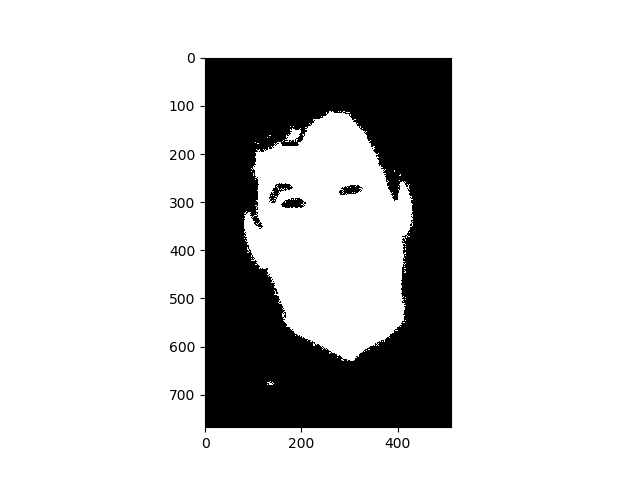
\includegraphics[width=\textwidth]{Task 2 Plots/bin_mask_006.png}
        \caption{image 006}
        \label{fig:binmask6}
    \end{subfigure}
    \begin{subfigure}{0.3\textwidth}
        \centering
        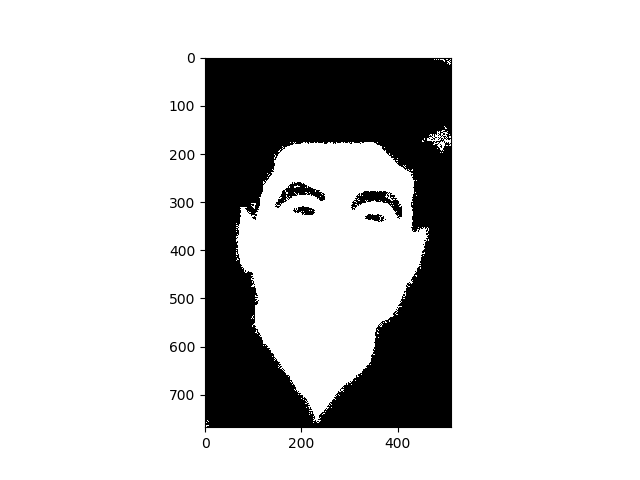
\includegraphics[width=\textwidth]{Task 2 Plots/bin_mask_007.png}
        \caption{image 007}
        \label{fig:binmask7}
    \end{subfigure}
    \begin{subfigure}{0.3\textwidth}
        \centering
        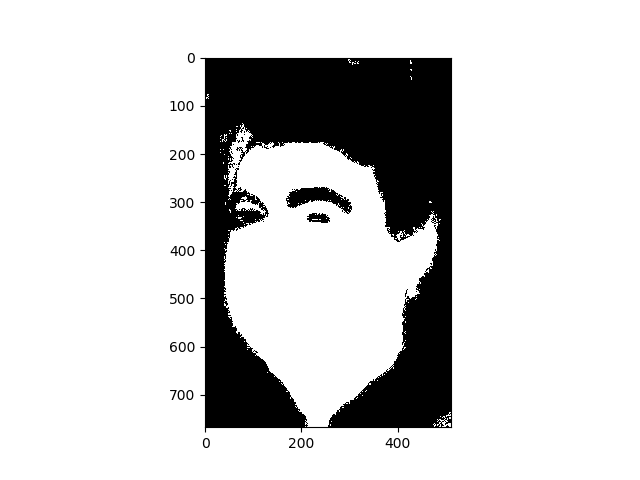
\includegraphics[width=\textwidth]{Task 2 Plots/bin_mask_008.png}
        \caption{image 008}
        \label{fig:binmask8}
    \end{subfigure}
    \begin{subfigure}{0.3\textwidth}
        \centering
        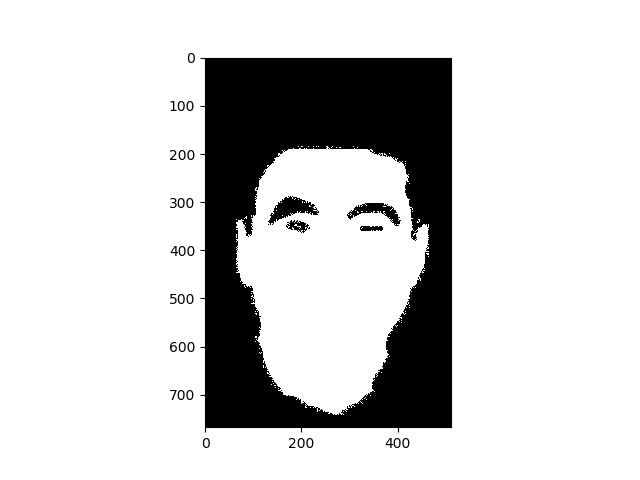
\includegraphics[width=\textwidth]{Task 2 Plots/bin_mask_009.png}
        \caption{image 009}
        \label{fig:binmask9}
    \end{subfigure}
    \begin{subfigure}{0.3\textwidth}
        \centering
        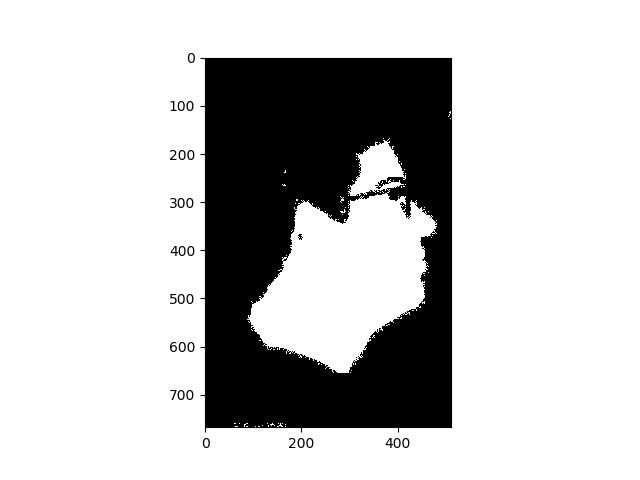
\includegraphics[width=\textwidth]{Task 2 Plots/bin_mask_010.png}
        \caption{image 010}
        \label{fig:binmask10}
    \end{subfigure}
    \caption{Binary Masks}
    \label{fig:binmasksall}
\end{figure}

\newpage

\section{Skin Color Segmentation}

In this part, I have determine a color range for skins by using binary masks that I have obtained in the first part. And in similar way to first part, I have created skin color masks.

\begin{figure}[H]
    \centering
    \begin{subfigure}{0.3\textwidth}
        \centering
        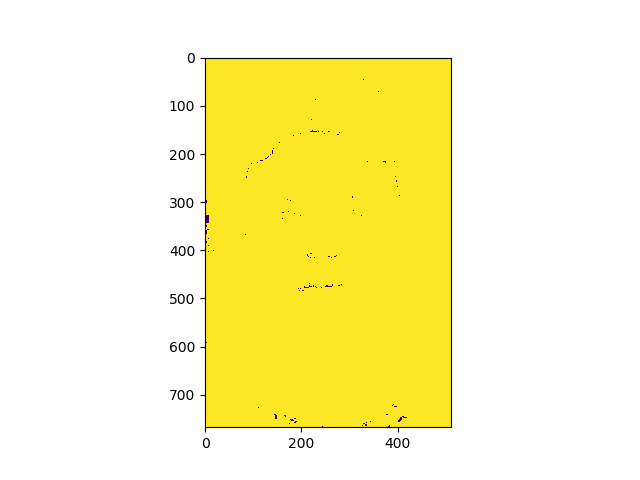
\includegraphics[width=\textwidth]{Task 2 Plots/skin_color_mask_001.png}
        \caption{image 001}
        \label{fig:skin_colormask1}
    \end{subfigure}
    \begin{subfigure}{0.3\textwidth}
        \centering
        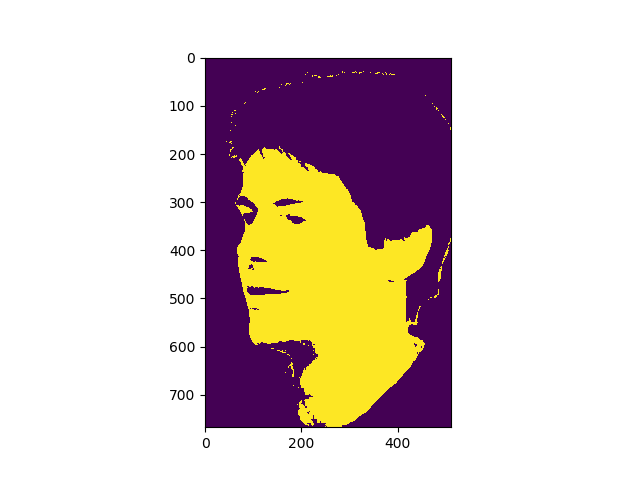
\includegraphics[width=\textwidth]{Task 2 Plots/skin_color_mask_002.png}
        \caption{image 002}
        \label{fig:skin_colormask2}
    \end{subfigure}
    \begin{subfigure}{0.3\textwidth}
        \centering
        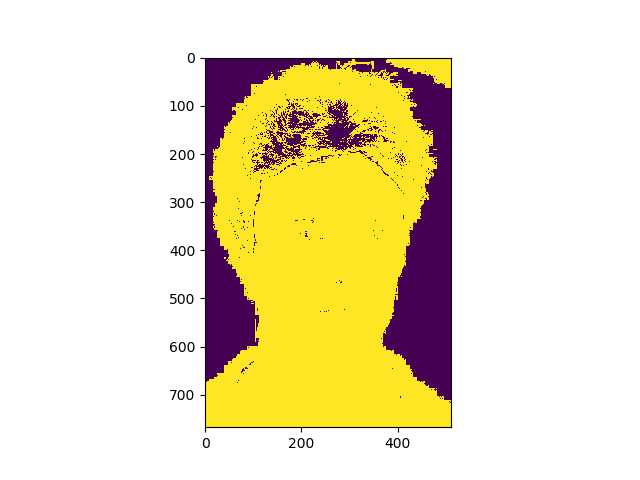
\includegraphics[width=\textwidth]{Task 2 Plots/skin_color_mask_003.png}
        \caption{image 003}
        \label{fig:skin_colormask3}
    \end{subfigure}
    \begin{subfigure}{0.3\textwidth}
        \centering
        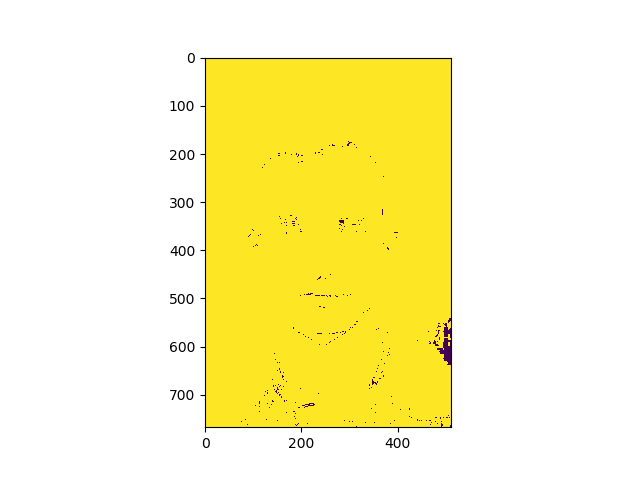
\includegraphics[width=\textwidth]{Task 2 Plots/skin_color_mask_004.png}
        \caption{image 004}
        \label{fig:skin_colormask4}
    \end{subfigure}
    \begin{subfigure}{0.3\textwidth}
        \centering
        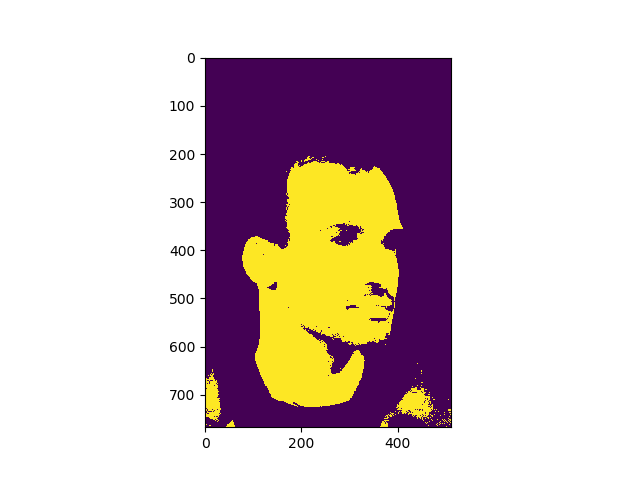
\includegraphics[width=\textwidth]{Task 2 Plots/skin_color_mask_005.png}
        \caption{image 005}
        \label{fig:skin_colormask5}
    \end{subfigure}
    \begin{subfigure}{0.3\textwidth}
        \centering
        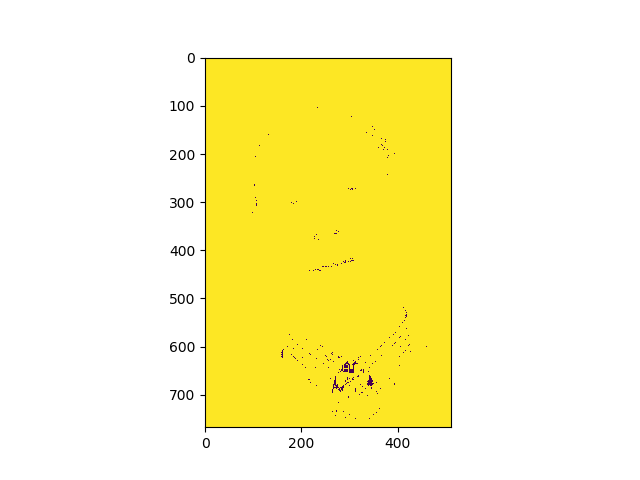
\includegraphics[width=\textwidth]{Task 2 Plots/skin_color_mask_006.png}
        \caption{image 006}
        \label{fig:skin_colormask6}
    \end{subfigure}
    \begin{subfigure}{0.3\textwidth}
        \centering
        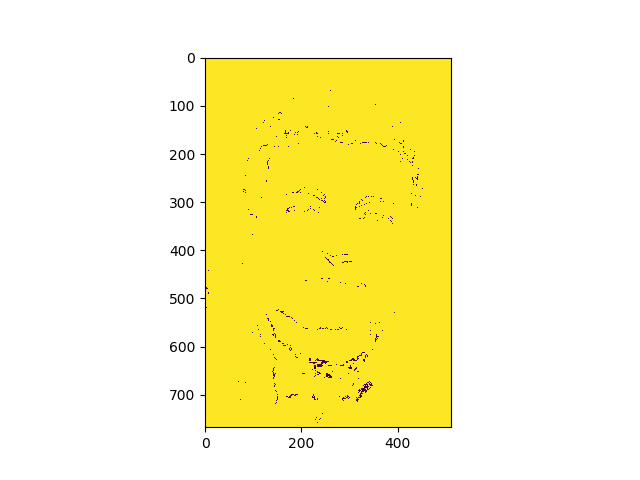
\includegraphics[width=\textwidth]{Task 2 Plots/skin_color_mask_007.png}
        \caption{image 007}
        \label{fig:skin_colormask7}
    \end{subfigure}
    \begin{subfigure}{0.3\textwidth}
        \centering
        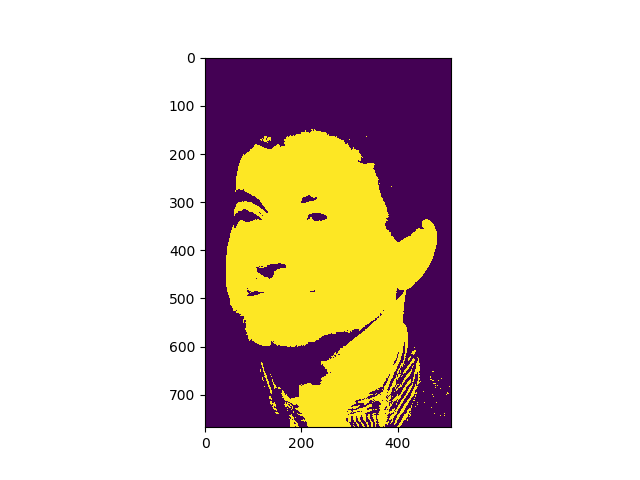
\includegraphics[width=\textwidth]{Task 2 Plots/skin_color_mask_008.png}
        \caption{image 008}
        \label{fig:skin_colormask8}
    \end{subfigure}
    \begin{subfigure}{0.3\textwidth}
        \centering
        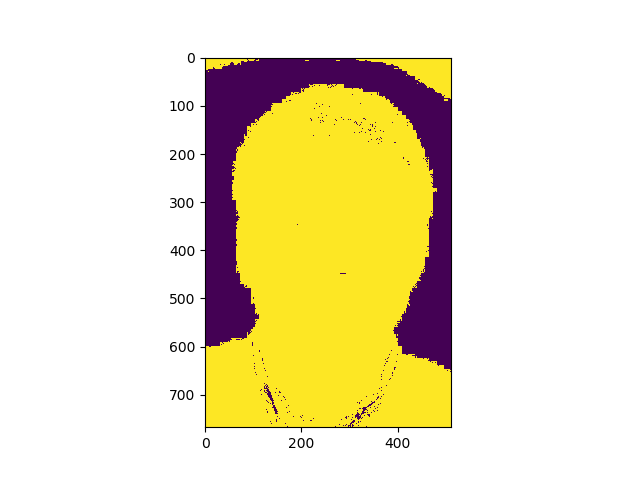
\includegraphics[width=\textwidth]{Task 2 Plots/skin_color_mask_009.png}
        \caption{image 009}
        \label{fig:skin_colormask9}
    \end{subfigure}
    \begin{subfigure}{0.3\textwidth}
        \centering
        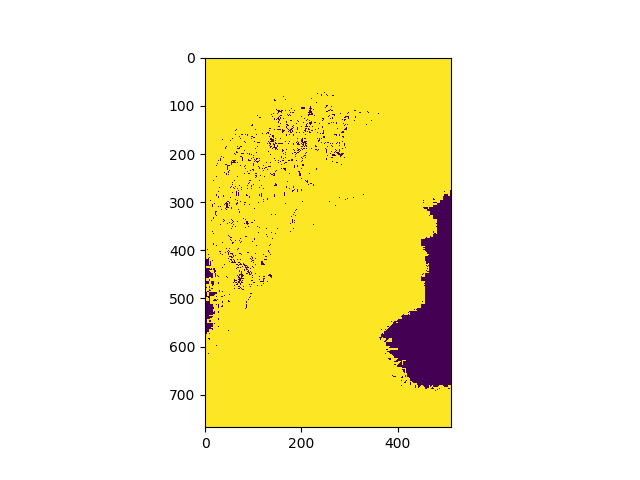
\includegraphics[width=\textwidth]{Task 2 Plots/skin_color_mask_010.png}
        \caption{image 010}
        \label{fig:skin_colormask10}
    \end{subfigure}
    \caption{Skin Color Masks}
    \label{fig:skincolormasksall}
\end{figure}

\newpage

As you can easily observe that, by using those binary masks, obtained ranges are working very bad. So in part 3, I have tried morphological operation "erosion" to get better masks, hence better skin color segmentation results.

\section{Skin Color Segmentation after Erosion}

For the last part of this task, I have eroded binary masks that I have obtained in first step. Then, repeated the skin color segmentation procedure. So, for binary masks results follows:

\begin{figure}[H]
    \centering
    \begin{subfigure}{0.4\textwidth}
        \centering
        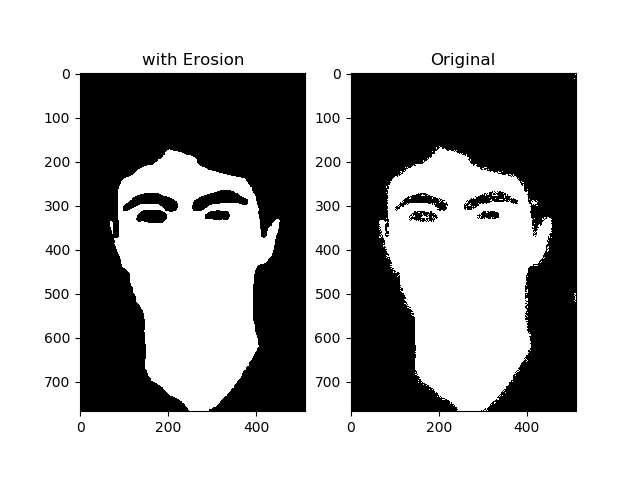
\includegraphics[width=\textwidth]{Task 2 Plots/bin_mask_erode_001.png}
        \caption{image 001}
        \label{fig:binmask_erode1}
    \end{subfigure}
    \begin{subfigure}{0.4\textwidth}
        \centering
        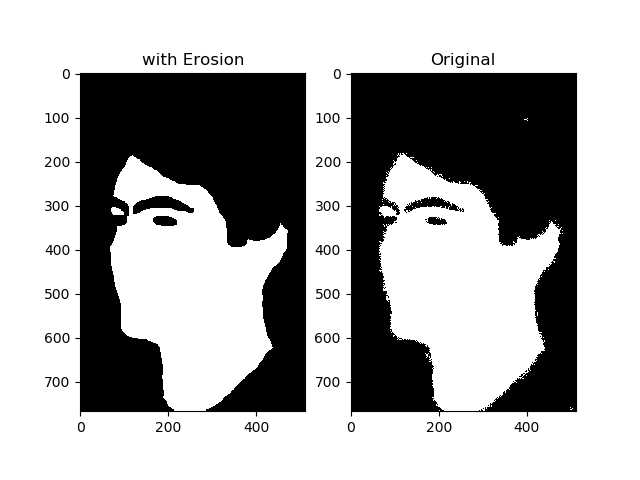
\includegraphics[width=\textwidth]{Task 2 Plots/bin_mask_erode_002.png}
        \caption{image 002}
        \label{fig:binmask_erode2}
    \end{subfigure}
    \begin{subfigure}{0.4\textwidth}
        \centering
        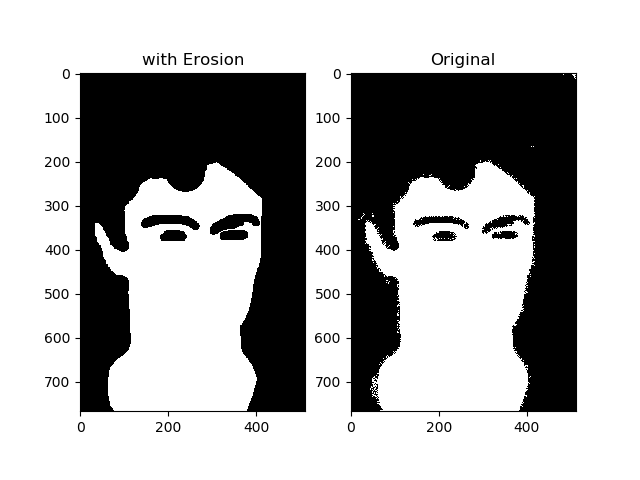
\includegraphics[width=\textwidth]{Task 2 Plots/bin_mask_erode_003.png}
        \caption{image 003}
        \label{fig:binmask_erode3}
    \end{subfigure}
    \begin{subfigure}{0.4\textwidth}
        \centering
        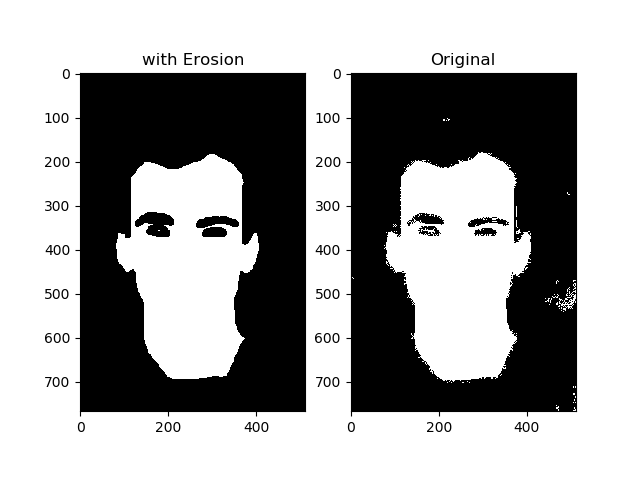
\includegraphics[width=\textwidth]{Task 2 Plots/bin_mask_erode_004.png}
        \caption{image 004}
        \label{fig:binmask_erode4}
    \end{subfigure}
    \begin{subfigure}{0.3\textwidth}
        \centering
        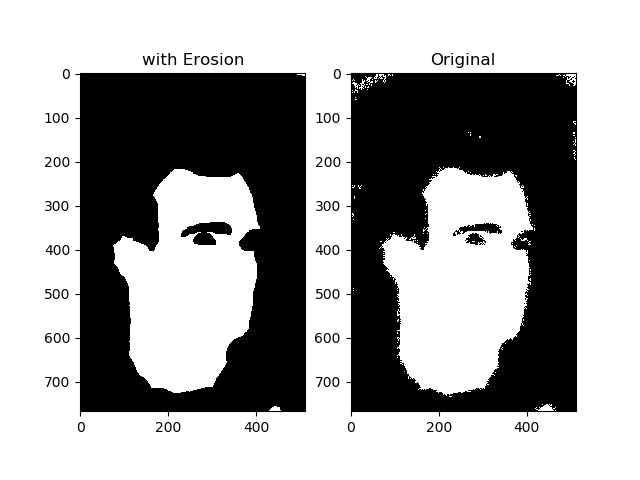
\includegraphics[width=\textwidth]{Task 2 Plots/bin_mask_erode_005.png}
        \caption{image 005}
        \label{fig:binmask_erode5}
    \end{subfigure}
    \begin{subfigure}{0.3\textwidth}
        \centering
        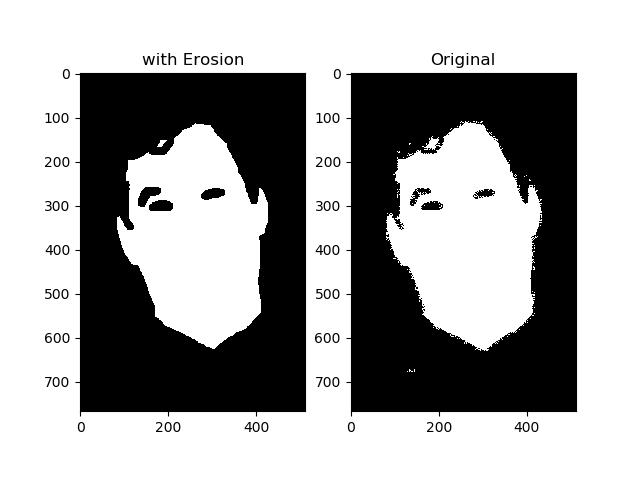
\includegraphics[width=\textwidth]{Task 2 Plots/bin_mask_erode_006.png}
        \caption{image 006}
        \label{fig:binmask_erode6}
    \end{subfigure}
    \begin{subfigure}{0.3\textwidth}
        \centering
        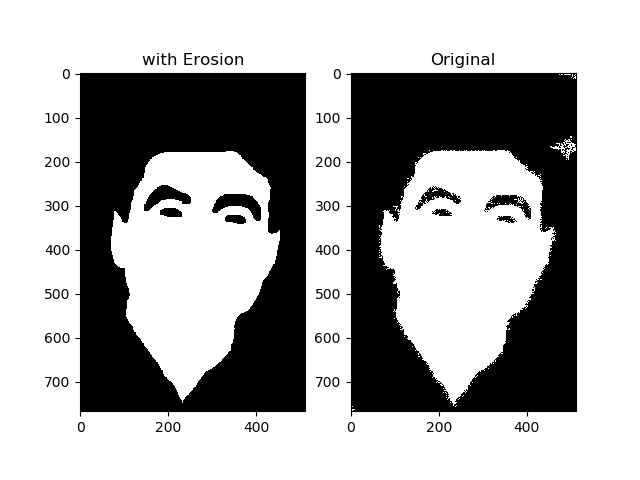
\includegraphics[width=\textwidth]{Task 2 Plots/bin_mask_erode_007.png}
        \caption{image 007}
        \label{fig:binmask_erode7}
    \end{subfigure}
    \begin{subfigure}{0.3\textwidth}
        \centering
        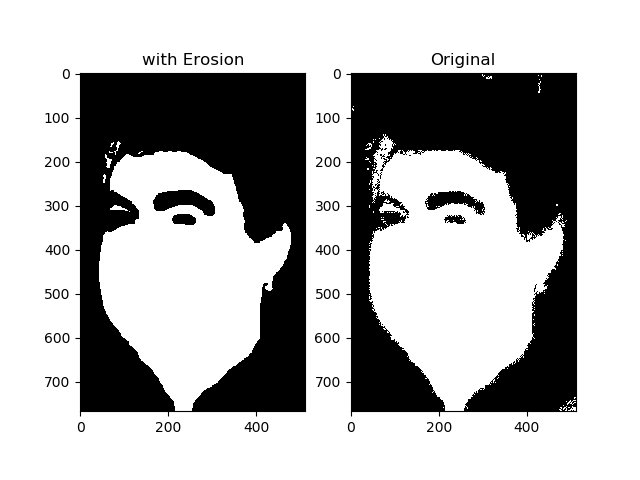
\includegraphics[width=\textwidth]{Task 2 Plots/bin_mask_erode_008.png}
        \caption{image 008}
        \label{fig:binmask_erode8}
    \end{subfigure}
    \begin{subfigure}{0.3\textwidth}
        \centering
        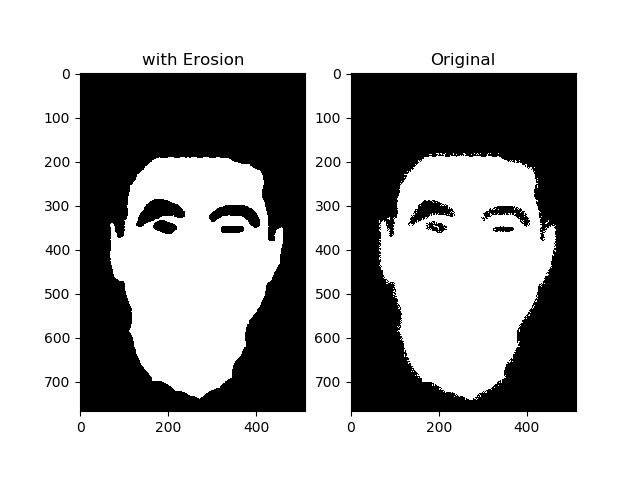
\includegraphics[width=\textwidth]{Task 2 Plots/bin_mask_erode_009.png}
        \caption{image 009}
        \label{fig:binmask_erode9}
    \end{subfigure}
    \begin{subfigure}{0.3\textwidth}
        \centering
        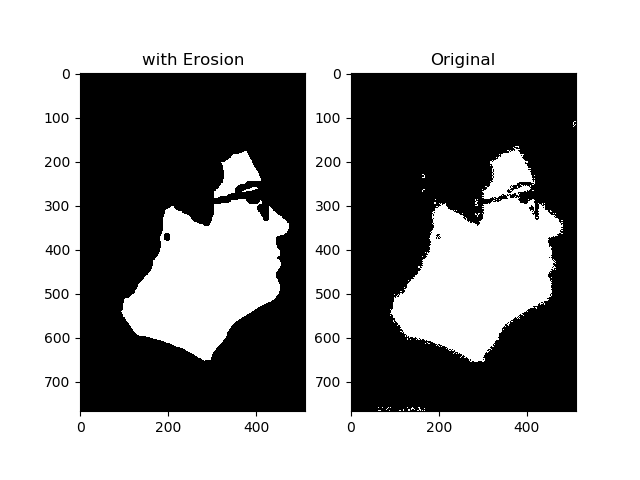
\includegraphics[width=\textwidth]{Task 2 Plots/bin_mask_erode_010.png}
        \caption{image 010}
        \label{fig:binmask_erode10}
    \end{subfigure}
    \caption{Eroded Binary Masks}
    \label{fig:binmaskerodedall}
\end{figure}

And resulting skin color masks follow:

\begin{figure}[H]
    \centering
    \begin{subfigure}{0.4\textwidth}
        \centering
        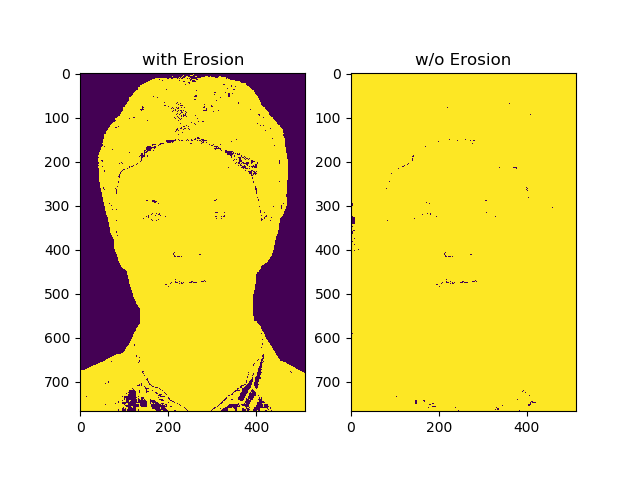
\includegraphics[width=\textwidth]{Task 2 Plots/skin_color_mask_erode_001.png}
        \caption{image 001}
        \label{fig:skin_colormask_erode1}
    \end{subfigure}
    \begin{subfigure}{0.4\textwidth}
        \centering
        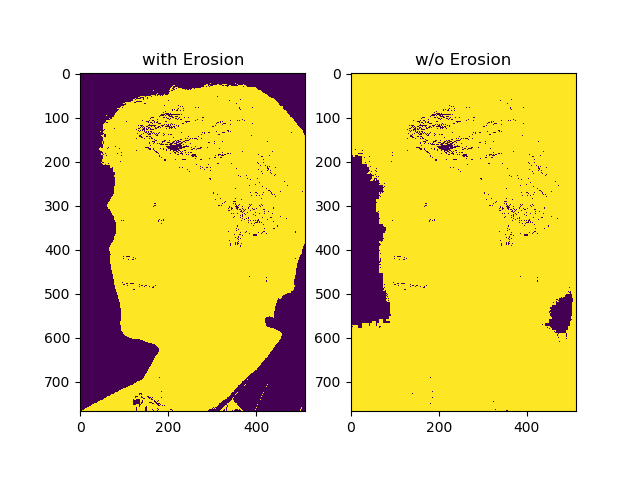
\includegraphics[width=\textwidth]{Task 2 Plots/skin_color_mask_erode_002.png}
        \caption{image 002}
        \label{fig:skin_colormask_erode2}
    \end{subfigure}
    \begin{subfigure}{0.4\textwidth}
        \centering
        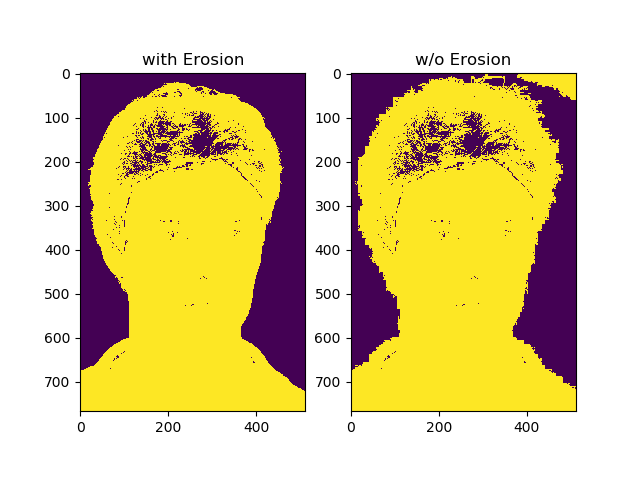
\includegraphics[width=\textwidth]{Task 2 Plots/skin_color_mask_erode_003.png}
        \caption{image 003}
        \label{fig:skin_colormask_erode3}
    \end{subfigure}
    \begin{subfigure}{0.4\textwidth}
        \centering
        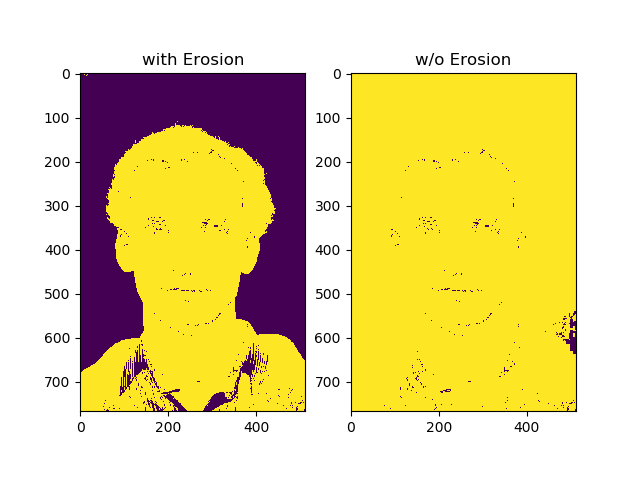
\includegraphics[width=\textwidth]{Task 2 Plots/skin_color_mask_erode_004.png}
        \caption{image 004}
        \label{fig:skin_colormask_erode4}
    \end{subfigure}
    \begin{subfigure}{0.3\textwidth}
        \centering
        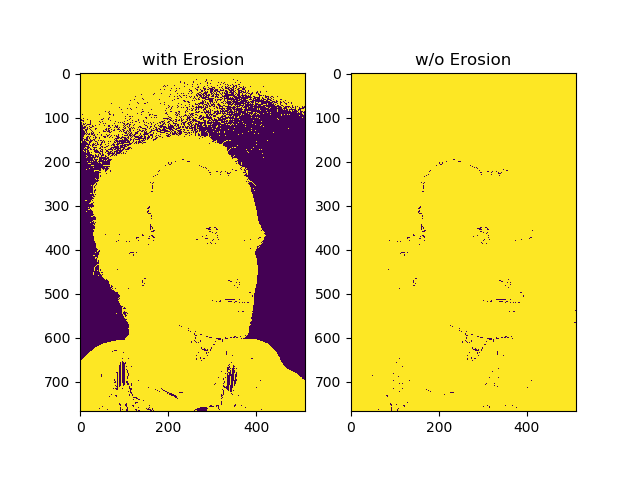
\includegraphics[width=\textwidth]{Task 2 Plots/skin_color_mask_erode_005.png}
        \caption{image 005}
        \label{fig:skin_colormask_erode5}
    \end{subfigure}
    \begin{subfigure}{0.3\textwidth}
        \centering
        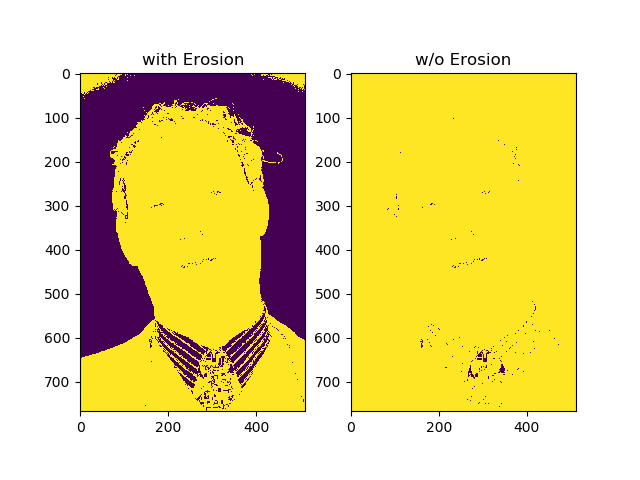
\includegraphics[width=\textwidth]{Task 2 Plots/skin_color_mask_erode_006.png}
        \caption{image 006}
        \label{fig:skin_colormask_erode6}
    \end{subfigure}
    \begin{subfigure}{0.3\textwidth}
        \centering
        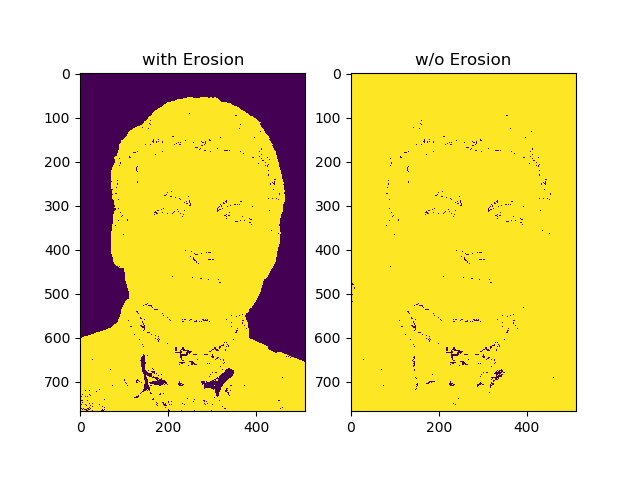
\includegraphics[width=\textwidth]{Task 2 Plots/skin_color_mask_erode_007.png}
        \caption{image 007}
        \label{fig:skin_colormask_erode7}
    \end{subfigure}
    \begin{subfigure}{0.3\textwidth}
        \centering
        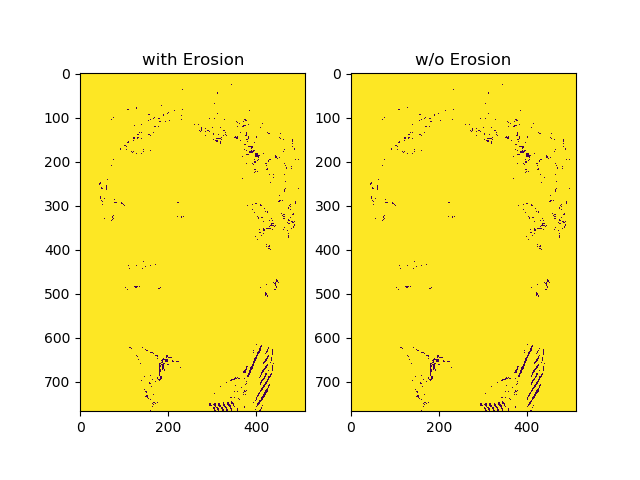
\includegraphics[width=\textwidth]{Task 2 Plots/skin_color_mask_erode_008.png}
        \caption{image 008}
        \label{fig:skin_colormask_erode8}
    \end{subfigure}
    \begin{subfigure}{0.3\textwidth}
        \centering
        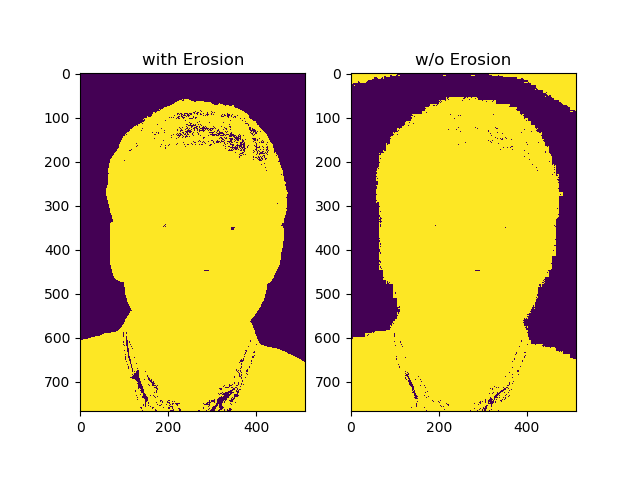
\includegraphics[width=\textwidth]{Task 2 Plots/skin_color_mask_erode_009.png}
        \caption{image 009}
        \label{fig:skin_colormask_erode9}
    \end{subfigure}
    \begin{subfigure}{0.3\textwidth}
        \centering
        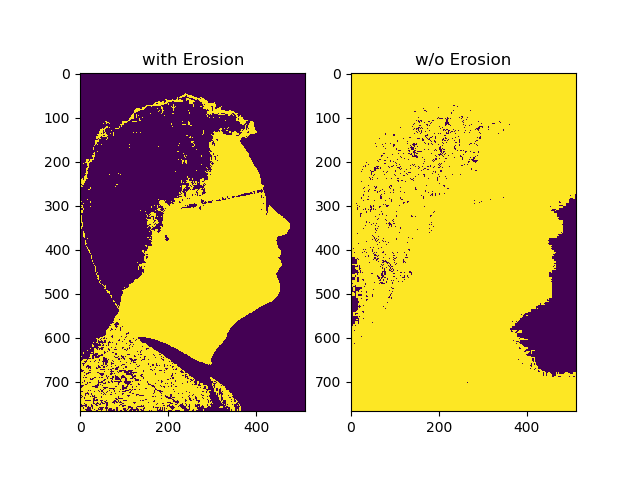
\includegraphics[width=\textwidth]{Task 2 Plots/skin_color_mask_erode_010.png}
        \caption{image 010}
        \label{fig:skin_colormask_erode10}
    \end{subfigure}
    \caption{Skin Color Masks with-w/o Erosion}
    \label{fig:skincolormaskerodedsall}
\end{figure}

\section{Conclusion}

For this part, I have realized that morphological operations might be very useful to eliminate noises from the image in such operations.

\chapter{Task 3}

\section{K-Means Algorithm}

K-Means is an unsupervised clustering algorithm. For this assignment, I have implemented K-Means similar to Matrix Factorization technique. For detailed explanation of this, you can see the \href{https://github.com/atcemgil/notes/blob/master/Kmeans.ipynb}{GitHub notes} from A.Taylan Cemgil. I got center update rule of my k-means class from his notes.

\section{Obtaining Skin Clusters}

\subsection{First Attempt}

My first attempt to obtain skin clusters was to plot k-means clustering results for each image for k from 2 to 10. Let see the results,

\begin{figure}[H]
    \centering
    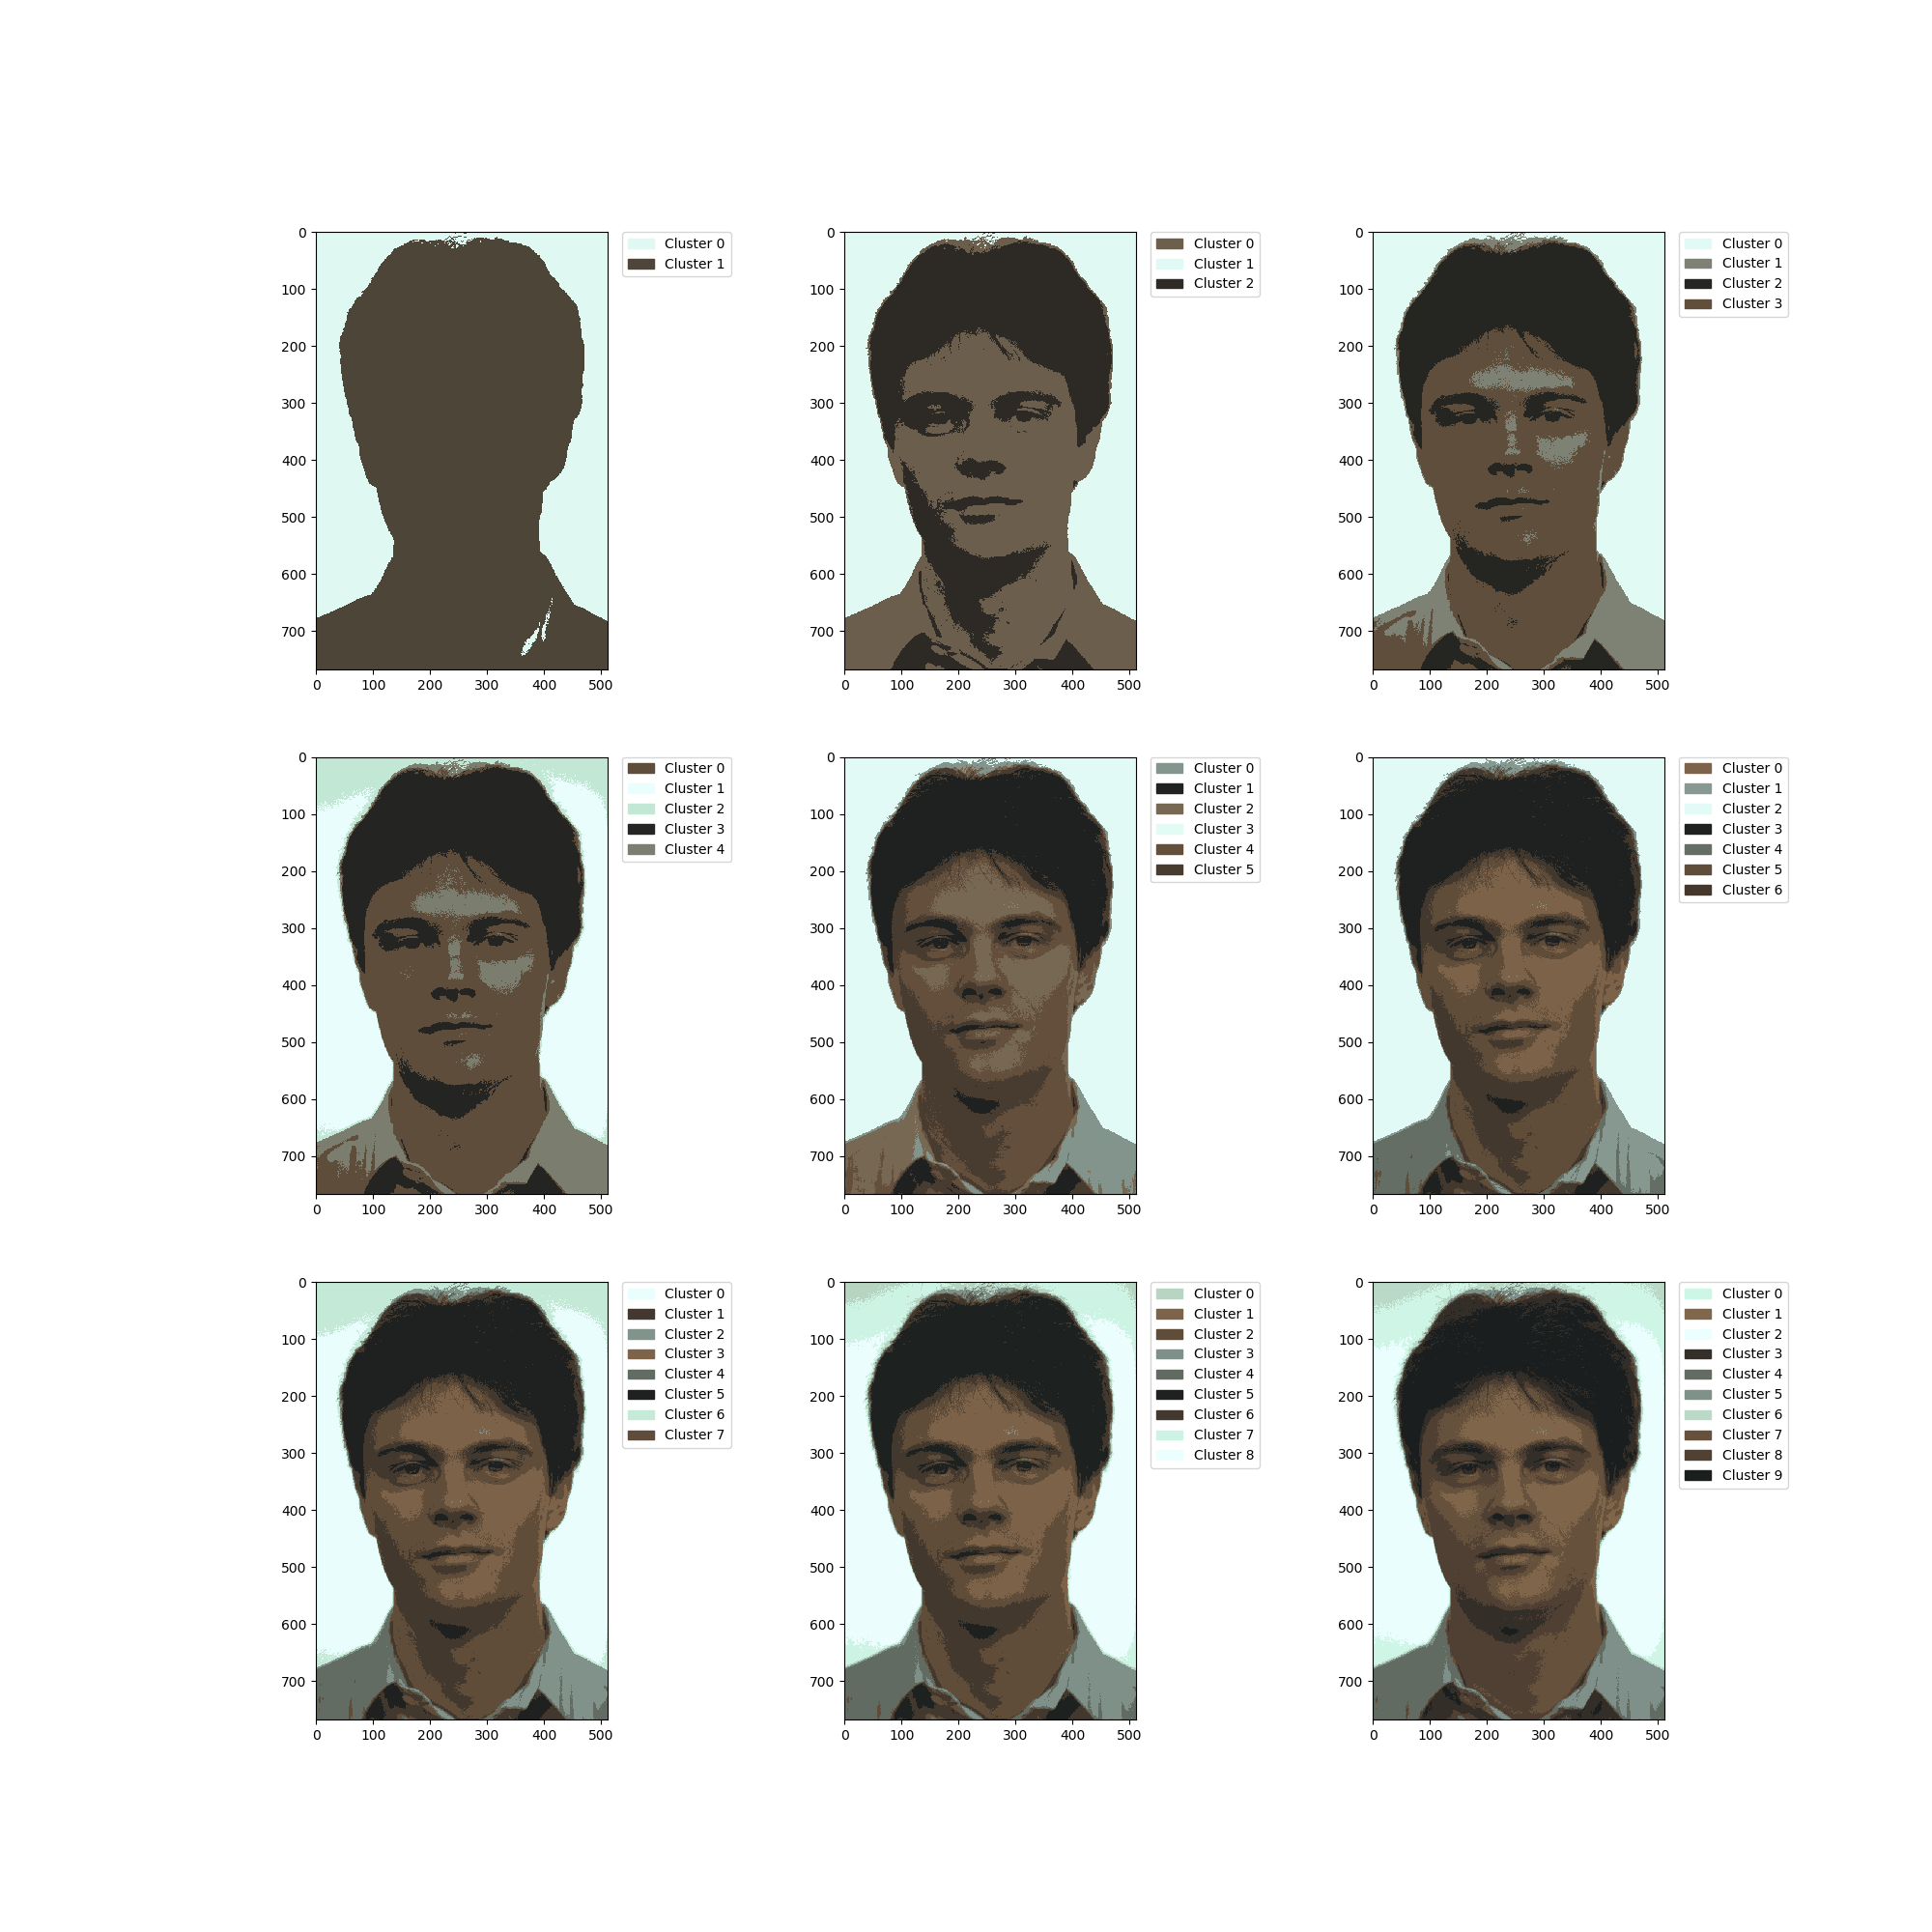
\includegraphics[width=0.9\textwidth, height=0.4\textheight]{Task 3 Plots/Clustering/clusters_001.png}
    \caption{Clustering Results for image 001}
    \label{fig:clusters1}
\end{figure}
\begin{figure}[H]
    \centering
    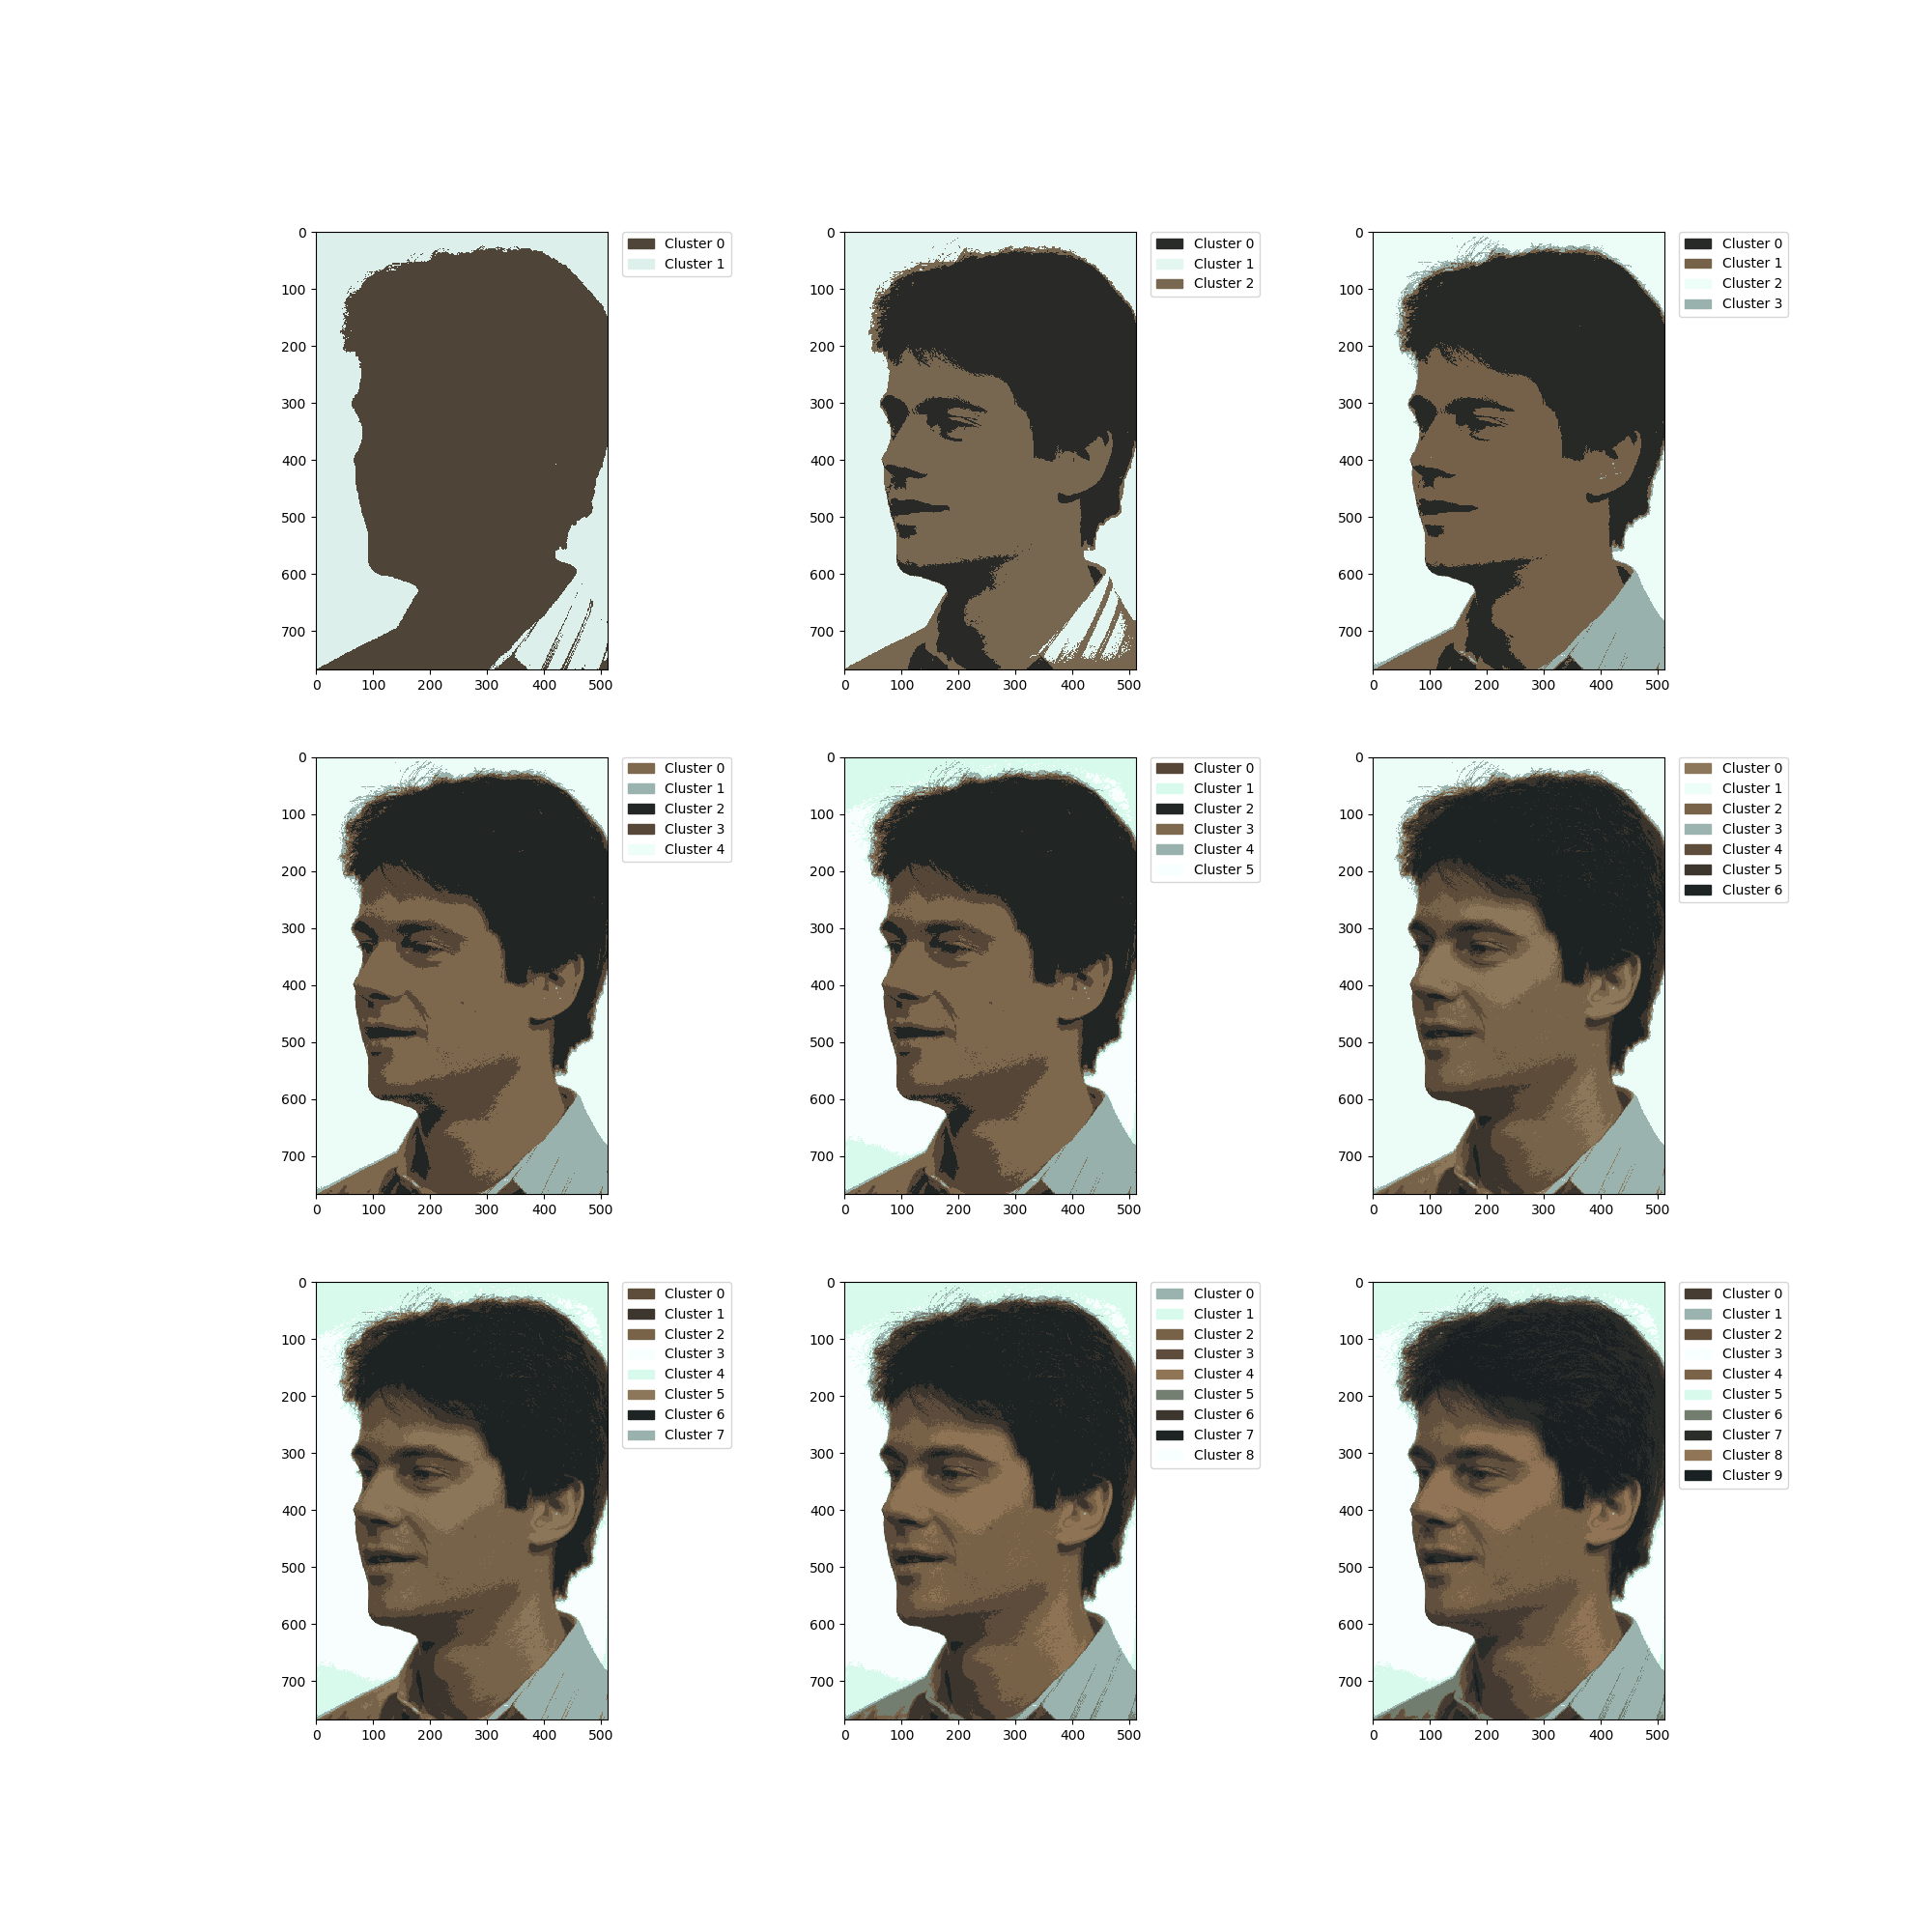
\includegraphics[width=0.9\textwidth, height=0.4\textheight]{Task 3 Plots/Clustering/clusters_002.png}
    \caption{Clustering Results for image 002}
    \label{fig:clusters2}
\end{figure}
\begin{figure}[H]
    \centering
    \includegraphics[width=0.9\textwidth, height=0.4\textheight]{Task 3 Plots/Clustering/clusters_003.png}
    \caption{Clustering Results for image 003}
    \label{fig:clusters3}
\end{figure}
\begin{figure}[H]
    \centering
    \includegraphics[width=0.9\textwidth, height=0.4\textheight]{Task 3 Plots/Clustering/clusters_004.png}
    \caption{Clustering Results for image 004}
    \label{fig:clusters4}
\end{figure}
\begin{figure}[H]
    \centering
    \includegraphics[width=0.9\textwidth, height=0.4\textheight]{Task 3 Plots/Clustering/clusters_005.png}
    \caption{Clustering Results for image 005}
    \label{fig:clusters5}
\end{figure}
\begin{figure}[H]
    \centering
    \includegraphics[width=0.9\textwidth, height=0.4\textheight]{Task 3 Plots/Clustering/clusters_006.png}
    \caption{Clustering Results for image 006}
    \label{fig:clusters6}
\end{figure}
\begin{figure}[H]
    \centering
    \includegraphics[width=0.9\textwidth, height=0.4\textheight]{Task 3 Plots/Clustering/clusters_007.png}
    \caption{Clustering Results for image 007}
    \label{fig:clusters7}
\end{figure}
\begin{figure}[H]
    \centering
    \includegraphics[width=0.9\textwidth, height=0.4\textheight]{Task 3 Plots/Clustering/clusters_008.png}
    \caption{Clustering Results for image 008}
    \label{fig:clusters8}
\end{figure}
\begin{figure}[H]
    \centering
    \includegraphics[width=0.9\textwidth, height=0.4\textheight]{Task 3 Plots/Clustering/clusters_009.png}
    \caption{Clustering Results for image 009}
    \label{fig:clusters9}
\end{figure}
\begin{figure}[H]
    \centering
    \includegraphics[width=0.9\textwidth, height=0.4\textheight]{Task 3 Plots/Clustering/clusters_010.png}
    \caption{Clustering Results for image 010}
    \label{fig:clusters10}
\end{figure}
\begin{figure}[H]
    \centering
    \includegraphics[width=0.9\textwidth, height=0.4\textheight]{Task 3 Plots/Clustering/clusters_011.png}
    \caption{Clustering Results for image 011}
    \label{fig:clusters11}
\end{figure}
\begin{figure}[H]
    \centering
    \includegraphics[width=0.9\textwidth, height=0.4\textheight]{Task 3 Plots/Clustering/clusters_012.png}
    \caption{Clustering Results for image 012}
    \label{fig:clusters12}
\end{figure}
\begin{figure}[H]
    \centering
    \includegraphics[width=0.9\textwidth, height=0.4\textheight]{Task 3 Plots/Clustering/clusters_013.png}
    \caption{Clustering Results for image 013}
    \label{fig:clusters13}
\end{figure}
\begin{figure}[H]
    \centering
    \includegraphics[width=0.9\textwidth, height=0.4\textheight]{Task 3 Plots/Clustering/clusters_014.png}
    \caption{Clustering Results for image 014}
    \label{fig:clusters14}
\end{figure}
\begin{figure}[H]
    \centering
    \includegraphics[width=0.9\textwidth, height=0.4\textheight]{Task 3 Plots/Clustering/clusters_015.png}
    \caption{Clustering Results for image 015}
    \label{fig:clusters15}
\end{figure}
\begin{figure}[H]
    \centering
    \includegraphics[width=0.9\textwidth, height=0.4\textheight]{Task 3 Plots/Clustering/clusters_016.png}
    \caption{Clustering Results for image 016}
    \label{fig:clusters16}
\end{figure}
\begin{figure}[H]
    \centering
    \includegraphics[width=0.9\textwidth, height=0.4\textheight]{Task 3 Plots/Clustering/clusters_017.png}
    \caption{Clustering Results for image 017}
    \label{fig:clusters17}
\end{figure}
\begin{figure}[H]
    \centering
    \includegraphics[width=0.9\textwidth, height=0.4\textheight]{Task 3 Plots/Clustering/clusters_018.png}
    \caption{Clustering Results for image 018}
    \label{fig:clusters18}
\end{figure}
\begin{figure}[H]
    \centering
    \includegraphics[width=0.9\textwidth, height=0.4\textheight]{Task 3 Plots/Clustering/clusters_019.png}
    \caption{Clustering Results for image 019}
    \label{fig:clusters19}
\end{figure}
\begin{figure}[H]
    \centering
    \includegraphics[width=0.9\textwidth, height=0.4\textheight]{Task 3 Plots/Clustering/clusters_020.png}
    \caption{Clustering Results for image 020}
    \label{fig:clusters20}
\end{figure}

After I plotted these images, I tried to select clusters that contains only skin pixels. But, it cannot be determined 100\% true. My second attempt to obtain these clusters was "Elbow Rule"

\subsection{Second Attempt: Elbow Rule}
\begin{figure}[H]
    \centering
    \begin{subfigure}{0.3\textwidth}
        \centering
        \includegraphics[width=0.9\textwidth]{Task 3 Plots/Elbow Plots/img_001.png}
        \caption{Elbow Rule for img 001}
        \label{fig:elbow1}
    \end{subfigure}
    \begin{subfigure}{0.3\textwidth}
        \centering
        \includegraphics[width=0.9\textwidth]{Task 3 Plots/Elbow Plots/img_002.png}
        \caption{Elbow Rule for img 002}
        \label{fig:elbow2}
    \end{subfigure}
    \begin{subfigure}{0.3\textwidth}
        \centering
        \includegraphics[width=0.9\textwidth]{Task 3 Plots/Elbow Plots/img_003.png}
        \caption{Elbow Rule for img 003}
        \label{fig:elbow3}
    \end{subfigure}
    \begin{subfigure}{0.3\textwidth}
        \centering
        \includegraphics[width=0.9\textwidth]{Task 3 Plots/Elbow Plots/img_004.png}
        \caption{Elbow Rule for img 004}
        \label{fig:elbow4}
    \end{subfigure}
    \begin{subfigure}{0.3\textwidth}
        \centering
        \includegraphics[width=0.9\textwidth]{Task 3 Plots/Elbow Plots/img_005.png}
        \caption{Elbow Rule for img 005}
        \label{fig:elbow5}
    \end{subfigure}
    \begin{subfigure}{0.3\textwidth}
        \centering
        \includegraphics[width=0.9\textwidth]{Task 3 Plots/Elbow Plots/img_006.png}
        \caption{Elbow Rule for img 006}
        \label{fig:elbow6}
    \end{subfigure}
    \begin{subfigure}{0.3\textwidth}
        \centering
        \includegraphics[width=0.9\textwidth]{Task 3 Plots/Elbow Plots/img_007.png}
        \caption{Elbow Rule for img 007}
        \label{fig:elbow7}
    \end{subfigure}
    \begin{subfigure}{0.3\textwidth}
        \centering
        \includegraphics[width=0.9\textwidth]{Task 3 Plots/Elbow Plots/img_008.png}
        \caption{Elbow Rule for img 008}
        \label{fig:elbow8}
    \end{subfigure}
    \begin{subfigure}{0.3\textwidth}
        \centering
        \includegraphics[width=0.9\textwidth]{Task 3 Plots/Elbow Plots/img_009.png}
        \caption{Elbow Rule for img 009}
        \label{fig:elbow9}
    \end{subfigure}
    \begin{subfigure}{0.3\textwidth}
        \centering
        \includegraphics[width=0.9\textwidth]{Task 3 Plots/Elbow Plots/img_010.png}
        \caption{Elbow Rule for img 010}
        \label{fig:elbow10}
    \end{subfigure}
\end{figure}
\begin{figure}[H] \ContinuedFloat
    \centering
    \begin{subfigure}{0.3\textwidth}
        \centering
        \includegraphics[width=0.9\textwidth]{Task 3 Plots/Elbow Plots/img_011.png}
        \caption{Elbow Rule for img 011}
        \label{fig:elbow11}
    \end{subfigure}
    \begin{subfigure}{0.3\textwidth}
        \centering
        \includegraphics[width=0.9\textwidth]{Task 3 Plots/Elbow Plots/img_012.png}
        \caption{Elbow Rule for img 012}
        \label{fig:elbow12}
    \end{subfigure}
    \begin{subfigure}{0.3\textwidth}
        \centering
        \includegraphics[width=0.9\textwidth]{Task 3 Plots/Elbow Plots/img_013.png}
        \caption{Elbow Rule for img 013}
        \label{fig:elbow13}
    \end{subfigure}
    \begin{subfigure}{0.3\textwidth}
        \centering
        \includegraphics[width=0.9\textwidth]{Task 3 Plots/Elbow Plots/img_014.png}
        \caption{Elbow Rule for img 014}
        \label{fig:elbow14}
    \end{subfigure}
    \begin{subfigure}{0.3\textwidth}
        \centering
        \includegraphics[width=0.9\textwidth]{Task 3 Plots/Elbow Plots/img_015.png}
        \caption{Elbow Rule for img 015}
        \label{fig:elbow15}
    \end{subfigure}
    \begin{subfigure}{0.3\textwidth}
        \centering
        \includegraphics[width=0.9\textwidth]{Task 3 Plots/Elbow Plots/img_016.png}
        \caption{Elbow Rule for img 016}
        \label{fig:elbow16}
    \end{subfigure}
    \begin{subfigure}{0.3\textwidth}
        \centering
        \includegraphics[width=0.9\textwidth]{Task 3 Plots/Elbow Plots/img_017.png}
        \caption{Elbow Rule for img 017}
        \label{fig:elbow17}
    \end{subfigure}
    \begin{subfigure}{0.3\textwidth}
        \centering
        \includegraphics[width=0.9\textwidth]{Task 3 Plots/Elbow Plots/img_018.png}
        \caption{Elbow Rule for img 018}
        \label{fig:elbow18}
    \end{subfigure}
    \begin{subfigure}{0.3\textwidth}
        \centering
        \includegraphics[width=0.9\textwidth]{Task 3 Plots/Elbow Plots/img_019.png}
        \caption{Elbow Rule for img 019}
        \label{fig:elbow19}
    \end{subfigure}
    \begin{subfigure}{0.3\textwidth}
        \centering
        \includegraphics[width=0.9\textwidth]{Task 3 Plots/Elbow Plots/img_020.png}
        \caption{Elbow Rule for img 020}
        \label{fig:elbow20}
    \end{subfigure}
    \caption{Elbow Rule Graphs}
    \label{fig:elbowall}
\end{figure}

After I plotted each of these graphs, I obtained cluster ids to obtain skin pixel masks. To get same cluster ids for same colors, I set numpy random seed as 58 just for fun.

\subsection{Results}

After trying 2 different approaches, I finally determined cluster ids for skin colors and obtained skin pixel masks for each image

\begin{figure}[H]
    \centering
    \begin{subfigure}{0.24\textwidth}
        \centering
        \includegraphics[width=\textwidth]{Task 3 Plots/Binary Masks/mask_001.png}
        \caption{Mask for image 001}
        \label{fig:kbinmask1}
    \end{subfigure}
    \begin{subfigure}{0.24\textwidth}
        \centering
        \includegraphics[width=\textwidth]{Task 3 Plots/Binary Masks/mask_002.png}
        \caption{Mask for image 002}
        \label{fig:kbinmask2}
    \end{subfigure}
    \begin{subfigure}{0.24\textwidth}
        \centering
        \includegraphics[width=\textwidth]{Task 3 Plots/Binary Masks/mask_003.png}
        \caption{Mask for image 003}
        \label{fig:kbinmask3}
    \end{subfigure}
    \begin{subfigure}{0.24\textwidth}
        \centering
        \includegraphics[width=\textwidth]{Task 3 Plots/Binary Masks/mask_004.png}
        \caption{Mask for image 004}
        \label{fig:kbinmask4}
    \end{subfigure}
    \begin{subfigure}{0.24\textwidth}
        \centering
        \includegraphics[width=\textwidth]{Task 3 Plots/Binary Masks/mask_005.png}
        \caption{Mask for image 005}
        \label{fig:kbinmask5}
    \end{subfigure}
    \begin{subfigure}{0.24\textwidth}
        \centering
        \includegraphics[width=\textwidth]{Task 3 Plots/Binary Masks/mask_006.png}
        \caption{Mask for image 006}
        \label{fig:kbinmask6}
    \end{subfigure}
    \begin{subfigure}{0.24\textwidth}
        \centering
        \includegraphics[width=\textwidth]{Task 3 Plots/Binary Masks/mask_007.png}
        \caption{Mask for image 007}
        \label{fig:kbinmask7}
    \end{subfigure}
    \begin{subfigure}{0.24\textwidth}
        \centering
        \includegraphics[width=\textwidth]{Task 3 Plots/Binary Masks/mask_008.png}
        \caption{Mask for image 008}
        \label{fig:kbinmask8}
    \end{subfigure}
    \begin{subfigure}{0.24\textwidth}
        \centering
        \includegraphics[width=\textwidth]{Task 3 Plots/Binary Masks/mask_009.png}
        \caption{Mask for image 009}
        \label{fig:kbinmask9}
    \end{subfigure}
    \begin{subfigure}{0.24\textwidth}
        \centering
        \includegraphics[width=\textwidth]{Task 3 Plots/Binary Masks/mask_010.png}
        \caption{Mask for image 010}
        \label{fig:kbinmask10}
    \end{subfigure}
    \begin{subfigure}{0.24\textwidth}
        \centering
        \includegraphics[width=\textwidth]{Task 3 Plots/Binary Masks/mask_011.png}
        \caption{Mask for image 011}
        \label{fig:kbinmask11}
    \end{subfigure}
    \begin{subfigure}{0.24\textwidth}
        \centering
        \includegraphics[width=\textwidth]{Task 3 Plots/Binary Masks/mask_012.png}
        \caption{Mask for image 012}
        \label{fig:kbinmask12}
    \end{subfigure}
    \begin{subfigure}{0.24\textwidth}
        \centering
        \includegraphics[width=\textwidth]{Task 3 Plots/Binary Masks/mask_013.png}
        \caption{Mask for image 013}
        \label{fig:kbinmask13}
    \end{subfigure}
    \begin{subfigure}{0.24\textwidth}
        \centering
        \includegraphics[width=\textwidth]{Task 3 Plots/Binary Masks/mask_014.png}
        \caption{Mask for image 014}
        \label{fig:kbinmask14}
    \end{subfigure}
    \begin{subfigure}{0.24\textwidth}
        \centering
        \includegraphics[width=\textwidth]{Task 3 Plots/Binary Masks/mask_015.png}
        \caption{Mask for image 015}
        \label{fig:kbinmask15}
    \end{subfigure}
    \begin{subfigure}{0.24\textwidth}
        \centering
        \includegraphics[width=\textwidth]{Task 3 Plots/Binary Masks/mask_016.png}
        \caption{Mask for image 016}
        \label{fig:kbinmask16}
    \end{subfigure}
    \begin{subfigure}{0.24\textwidth}
        \centering
        \includegraphics[width=\textwidth]{Task 3 Plots/Binary Masks/mask_017.png}
        \caption{Mask for image 017}
        \label{fig:kbinmask17}
    \end{subfigure}
    \begin{subfigure}{0.24\textwidth}
        \centering
        \includegraphics[width=\textwidth]{Task 3 Plots/Binary Masks/mask_018.png}
        \caption{Mask for image 018}
        \label{fig:kbinmask18}
    \end{subfigure}
    \begin{subfigure}{0.24\textwidth}
        \centering
        \includegraphics[width=\textwidth]{Task 3 Plots/Binary Masks/mask_019.png}
        \caption{Mask for image 019}
        \label{fig:kbinmask19}
    \end{subfigure}
    \begin{subfigure}{0.24\textwidth}
        \centering
        \includegraphics[width=\textwidth]{Task 3 Plots/Binary Masks/mask_020.png}
        \caption{Mask for image 020}
        \label{fig:kbinmask20}
    \end{subfigure}

    \caption{Results of obtained skin clusters}
    \label{fig:skinpixelmasksall}
\end{figure}

\section{Obtain Skin Color Mask by Skin Color Segmentation}

In this part, I have used skin color segmentation technique from task 2 to obtain following results,

\begin{figure}[H]
    \centering
    \begin{subfigure}{0.24\textwidth}
        \centering
        \includegraphics[width=\textwidth]{Task 3 Plots/Skin Color Masks/mask_001.png}
        \caption{Skin Color Mask for image 001}
        \label{fig:kskincolormask1}
    \end{subfigure}
    \begin{subfigure}{0.24\textwidth}
        \centering
        \includegraphics[width=\textwidth]{Task 3 Plots/Skin Color Masks/mask_002.png}
        \caption{Skin Color Mask for image 002}
        \label{fig:kskincolormask2}
    \end{subfigure}
    \begin{subfigure}{0.24\textwidth}
        \centering
        \includegraphics[width=\textwidth]{Task 3 Plots/Skin Color Masks/mask_003.png}
        \caption{Skin Color Mask for image 003}
        \label{fig:kskincolormask3}
    \end{subfigure}
    \begin{subfigure}{0.24\textwidth}
        \centering
        \includegraphics[width=\textwidth]{Task 3 Plots/Skin Color Masks/mask_004.png}
        \caption{Skin Color Mask for image 004}
        \label{fig:kskincolormask4}
    \end{subfigure}
    \begin{subfigure}{0.24\textwidth}
        \centering
        \includegraphics[width=\textwidth]{Task 3 Plots/Skin Color Masks/mask_005.png}
        \caption{Skin Color Mask for image 005}
        \label{fig:kskincolormask5}
    \end{subfigure}
    \begin{subfigure}{0.24\textwidth}
        \centering
        \includegraphics[width=\textwidth]{Task 3 Plots/Skin Color Masks/mask_006.png}
        \caption{Skin Color Mask for image 006}
        \label{fig:kskincolormask6}
    \end{subfigure}
    \begin{subfigure}{0.24\textwidth}
        \centering
        \includegraphics[width=\textwidth]{Task 3 Plots/Skin Color Masks/mask_007.png}
        \caption{Skin Color Mask for image 007}
        \label{fig:kskincolormask7}
    \end{subfigure}
    \begin{subfigure}{0.24\textwidth}
        \centering
        \includegraphics[width=\textwidth]{Task 3 Plots/Skin Color Masks/mask_008.png}
        \caption{Skin Color Mask for image 008}
        \label{fig:kskincolormask8}
    \end{subfigure}
    \begin{subfigure}{0.24\textwidth}
        \centering
        \includegraphics[width=\textwidth]{Task 3 Plots/Skin Color Masks/mask_009.png}
        \caption{Skin Color Mask for image 009}
        \label{fig:kskincolormask9}
    \end{subfigure}
    \begin{subfigure}{0.24\textwidth}
        \centering
        \includegraphics[width=\textwidth]{Task 3 Plots/Skin Color Masks/mask_010.png}
        \caption{Skin Color Mask for image 010}
        \label{fig:kskincolormask10}
    \end{subfigure}
    \begin{subfigure}{0.24\textwidth}
        \centering
        \includegraphics[width=\textwidth]{Task 3 Plots/Skin Color Masks/mask_011.png}
        \caption{Skin Color Mask for image 011}
        \label{fig:kskincolormask11}
    \end{subfigure}
    \begin{subfigure}{0.24\textwidth}
        \centering
        \includegraphics[width=\textwidth]{Task 3 Plots/Skin Color Masks/mask_012.png}
        \caption{Skin Color Mask for image 012}
        \label{fig:kskincolormask12}
    \end{subfigure}
    \begin{subfigure}{0.24\textwidth}
        \centering
        \includegraphics[width=\textwidth]{Task 3 Plots/Skin Color Masks/mask_013.png}
        \caption{Skin Color Mask for image 013}
        \label{fig:kskincolormask13}
    \end{subfigure}
    \begin{subfigure}{0.24\textwidth}
        \centering
        \includegraphics[width=\textwidth]{Task 3 Plots/Skin Color Masks/mask_014.png}
        \caption{Skin Color Mask for image 014}
        \label{fig:kskincolormask14}
    \end{subfigure}
    \begin{subfigure}{0.24\textwidth}
        \centering
        \includegraphics[width=\textwidth]{Task 3 Plots/Skin Color Masks/mask_015.png}
        \caption{Skin Color Mask for image 015}
        \label{fig:kskincolormask15}
    \end{subfigure}
    \begin{subfigure}{0.24\textwidth}
        \centering
        \includegraphics[width=\textwidth]{Task 3 Plots/Skin Color Masks/mask_016.png}
        \caption{Skin Color Mask for image 016}
        \label{fig:kskincolormask16}
    \end{subfigure}
    \begin{subfigure}{0.24\textwidth}
        \centering
        \includegraphics[width=\textwidth]{Task 3 Plots/Skin Color Masks/mask_017.png}
        \caption{Skin Color Mask for image 017}
        \label{fig:kskincolormask17}
    \end{subfigure}
    \begin{subfigure}{0.24\textwidth}
        \centering
        \includegraphics[width=\textwidth]{Task 3 Plots/Skin Color Masks/mask_018.png}
        \caption{Skin Color Mask for image 018}
        \label{fig:kskincolormask18}
    \end{subfigure}
    \begin{subfigure}{0.24\textwidth}
        \centering
        \includegraphics[width=\textwidth]{Task 3 Plots/Skin Color Masks/mask_019.png}
        \caption{Skin Color Mask for image 019}
        \label{fig:kskincolormask19}
    \end{subfigure}
    \begin{subfigure}{0.24\textwidth}
        \centering
        \includegraphics[width=\textwidth]{Task 3 Plots/Skin Color Masks/mask_020.png}
        \caption{Skin Color Mask for image 020}
        \label{fig:kskincolormask20}
    \end{subfigure}
    \caption{Skin Color Masks Obtained by Binary Mask results of k-Means Clustering}
    \label{fig:ksincolormaskall}
\end{figure}

\section{Results and Future Improvements}

As everybody can obtain, using min-max range values to detect skin colors are not working well. To improve results of skin color segmentation, we can apply several techniques. First thing that came up is to increase cluster numbers in k-Means clustering so every skin pixel can separately obtained, but this is computationally heavy.

The second thing is to improve segmentation part. For this, we can think our skin color segmentation mechanism as a classifier which classifies between skin colors and non-skin colors. Using min-max as a classifier is a very naive approach. We can do following things;

\begin{itemize}[label=\ding{212}]
\item First, by using binary masks, we can constructs data set such that each skin pixel corresponds to 1, and non-skin pixel corresponds to 0 label
\item Second, we should split data set in 2 parts train and label
\item Then, we can train a binary classifier with train data set
\item Test it with test data set
\item Apply classifier to image colors
\item Based on classifier results we can obtain a skin color mask for the image
\end{itemize}

\subsection{Results}

Let see the segmentation results from logistic regression classifier,

\begin{figure}
    \centering
    \begin{subfigure}{0.24\textwidth}
        \centering
        \includegraphics[width=\textwidth]{Task 3 Plots/Logistic Regression Results/skin_color_mask_001.png}
        \caption{image 001}
        \label{fig:lskincolormask1}
    \end{subfigure}
    \begin{subfigure}{0.24\textwidth}
        \centering
        \includegraphics[width=\textwidth]{Task 3 Plots/Logistic Regression Results/skin_color_mask_002.png}
        \caption{image 002}
        \label{fig:lskincolormask2}
    \end{subfigure}
    \begin{subfigure}{0.24\textwidth}
        \centering
        \includegraphics[width=\textwidth]{Task 3 Plots/Logistic Regression Results/skin_color_mask_003.png}
        \caption{image 003}
        \label{fig:lskincolormask3}
    \end{subfigure}
    \begin{subfigure}{0.24\textwidth}
        \centering
        \includegraphics[width=\textwidth]{Task 3 Plots/Logistic Regression Results/skin_color_mask_004.png}
        \caption{image 004}
        \label{fig:lskincolormask4}
    \end{subfigure}
    \begin{subfigure}{0.24\textwidth}
        \centering
        \includegraphics[width=\textwidth]{Task 3 Plots/Logistic Regression Results/skin_color_mask_005.png}
        \caption{image 005}
        \label{fig:lskincolormask5}
    \end{subfigure}
    \begin{subfigure}{0.24\textwidth}
        \centering
        \includegraphics[width=\textwidth]{Task 3 Plots/Logistic Regression Results/skin_color_mask_006.png}
        \caption{image 006}
        \label{fig:lskincolormask6}
    \end{subfigure}
    \begin{subfigure}{0.24\textwidth}
        \centering
        \includegraphics[width=\textwidth]{Task 3 Plots/Logistic Regression Results/skin_color_mask_007.png}
        \caption{image 007}
        \label{fig:lskincolormask7}
    \end{subfigure}
    \begin{subfigure}{0.24\textwidth}
        \centering
        \includegraphics[width=\textwidth]{Task 3 Plots/Logistic Regression Results/skin_color_mask_008.png}
        \caption{image 008}
        \label{fig:lskincolormask8}
    \end{subfigure}
    \begin{subfigure}{0.24\textwidth}
        \centering
        \includegraphics[width=\textwidth]{Task 3 Plots/Logistic Regression Results/skin_color_mask_009.png}
        \caption{image 009}
        \label{fig:lskincolormask9}
    \end{subfigure}
    \begin{subfigure}{0.24\textwidth}
        \centering
        \includegraphics[width=\textwidth]{Task 3 Plots/Logistic Regression Results/skin_color_mask_010.png}
        \caption{image 010}
        \label{fig:lskincolormask10}
    \end{subfigure}
    \begin{subfigure}{0.24\textwidth}
        \centering
        \includegraphics[width=\textwidth]{Task 3 Plots/Logistic Regression Results/skin_color_mask_011.png}
        \caption{image 011}
        \label{fig:lskincolormask11}
    \end{subfigure}
    \begin{subfigure}{0.24\textwidth}
        \centering
        \includegraphics[width=\textwidth]{Task 3 Plots/Logistic Regression Results/skin_color_mask_012.png}
        \caption{image 012}
        \label{fig:lskincolormask12}
    \end{subfigure}
    \begin{subfigure}{0.24\textwidth}
        \centering
        \includegraphics[width=\textwidth]{Task 3 Plots/Logistic Regression Results/skin_color_mask_013.png}
        \caption{image 013}
        \label{fig:lskincolormask13}
    \end{subfigure}
    \begin{subfigure}{0.24\textwidth}
        \centering
        \includegraphics[width=\textwidth]{Task 3 Plots/Logistic Regression Results/skin_color_mask_014.png}
        \caption{image 014}
        \label{fig:lskincolormask14}
    \end{subfigure}
    \begin{subfigure}{0.24\textwidth}
        \centering
        \includegraphics[width=\textwidth]{Task 3 Plots/Logistic Regression Results/skin_color_mask_015.png}
        \caption{image 015}
        \label{fig:lskincolormask15}
    \end{subfigure}
    \begin{subfigure}{0.24\textwidth}
        \centering
        \includegraphics[width=\textwidth]{Task 3 Plots/Logistic Regression Results/skin_color_mask_016.png}
        \caption{image 016}
        \label{fig:lskincolormask16}
    \end{subfigure}
    \begin{subfigure}{0.24\textwidth}
        \centering
        \includegraphics[width=\textwidth]{Task 3 Plots/Logistic Regression Results/skin_color_mask_017.png}
        \caption{image 017}
        \label{fig:lskincolormask17}
    \end{subfigure}
    \begin{subfigure}{0.24\textwidth}
        \centering
        \includegraphics[width=\textwidth]{Task 3 Plots/Logistic Regression Results/skin_color_mask_018.png}
        \caption{image 018}
        \label{fig:lskincolormask18}
    \end{subfigure}
    \begin{subfigure}{0.24\textwidth}
        \centering
        \includegraphics[width=\textwidth]{Task 3 Plots/Logistic Regression Results/skin_color_mask_019.png}
        \caption{image 019}
        \label{fig:lskincolormask19}
    \end{subfigure}
    \begin{subfigure}{0.24\textwidth}
        \centering
        \includegraphics[width=\textwidth]{Task 3 Plots/Logistic Regression Results/skin_color_mask_020.png}
        \caption{image 020}
        \label{fig:lskincolormask20}
    \end{subfigure}
    
    \caption{Logistic Regression Results}
    \label{fig:logregressionall}
\end{figure}

\chapter{References}

\begin{itemize}
    \item \href{https://staff.fnwi.uva.nl/r.vandenboomgaard/IPCV20162017/20162017/LabExercises/SkinColorDetection.html}{Logistic Regression Approach to Skin Color Segmentation}
    \item \href{https://github.com/atcemgil/notes/blob/master/Kmeans.ipynb}{k-Means notes from A.Taylan Cemgil GitHub page}
\end{itemize}
\end{document}